%% 
%% Copyright 2019-2020 Elsevier Ltd
%% 
%% This file is part of the 'CAS Bundle'.
%% --------------------------------------
%% 
%% It may be distributed under the conditions of the LaTeX Project Public
%% License, either version 1.2 of this license or (at your option) any
%% later version.  The latest version of this license is in
%%    http://www.latex-project.org/lppl.txt
%% and version 1.2 or later is part of all distributions of LaTeX
%% version 1999/12/01 or later.
%% 
%% The list of all files belonging to the 'CAS Bundle' is
%% given in the file `manifest.txt'.
%% 
%% Template article for cas-sc documentclass for 
%% double column output.

%\documentclass[a4paper,fleqn,longmktitle]{cas-sc}
\documentclass[a4paper,fleqn]{cas-sc}

% \usepackage[numbers]{natbib}
%\usepackage[authoryear]{natbib}
\usepackage[authoryear,longnamesfirst]{natbib}
\usepackage{amssymb}
\usepackage{pifont}
\usepackage[section]{placeins} % oppure senza [section]

\newcommand{\cmark}{\ding{51}}  % ✓
\newcommand{\xmark}{\ding{55}}  % ✗                
\usepackage{svg}
\usepackage{booktabs}         
\usepackage{array} 
\usepackage[table]{xcolor}   % colori nelle celle     
%% The amsmath package provides various useful equation environments.
\usepackage{amsmath}
%% The amsthm package provides extended theorem environments
%% \usepackage{amsthm}
%% The lineno packages adds line numbers. Start line numbering with
%% \begin{linenumbers}, end it with \end{linenumbers}. Or switch it on
%% for the whole article with \linenumbers.
\usepackage{lineno}
\usepackage{pdfpages}

\usepackage[utf8]{inputenc}
\usepackage[T1]{fontenc}

%\usepackage{array}
\usepackage{enumitem}
\usepackage{makecell}
%\usepackage{geometry}
%\usepackage{booktabs}
\usepackage{graphicx}
\usepackage{tabularx}
\usepackage{comment}
\usepackage{tabularray}
%\usepackage{pdflscape} 
\usepackage{multirow}
\usepackage{hhline}
\usepackage{rotating}
\usepackage{colortbl}
\usepackage{float}
\usepackage{subcaption}
\usepackage{pdfpages}
\usepackage{changepage}
%\usepackage{enumerate}
%\usepackage[table,xcdraw]{xcolor}  
\usepackage{url}
\usepackage[scaled]{helvet}
%\usepackage{color} 

\usepackage{cancel}
% Beamer presentation requires \usepackage{colortbl} instead of
\usepackage[normalem]{ulem}
\usepackage{booktabs}
\usepackage{longtable}
\usepackage{multirow}
\usepackage{graphicx}  
\usepackage{booktabs,tabularx}
\usepackage{hyperref}
\newcommand{\sid}[1]{\hyperlink{#1}{#1}}
\def\UrlBreaks{\do\/\do-}

\newcommand{\DD}[2]{\textcolor{blue}{#1}[\textcolor{red}{#2}]}
\newcommand{\GM}[2]{\textcolor{red}{#1}[\textcolor{teal}{#2}]}
\newcommand{\NC}[2]{\textcolor{olive}{#1}[\textcolor{olive}{#2}]}
\newcommand{\SA}[2]{\textcolor{olive}{#1}[\textcolor{magenta}{#2}]}

%\newcommand{\PSRQone}{PS-RQ1: What kind and how many primary studies have been identified per publication year?}
\newcommand{\PSRQone}{RQ1: How are the primary studies distributed by venue type and publication year?}
%\newcommand{\PSRQtwo}{PS-RQ2: What are the venues and areas of interest of the primary studies that have been published?}
\newcommand{\PSRQtwo}{RQ2: What are the venues where the primary studies have been published?}
%\newcommand{\PSRQthree}{PS-RQ3: What are the authors’ affiliation countries of the selected primary studies?}
\newcommand{\PSRQthree}{RQ3: How are primary studies distributed across authors’ affiliation countries?}

\newcommand{\RSRQone}{RQ1: What are the adopted definitions of customer churn?}
\newcommand{\RSRQtwo}{RQ2: What features have been used for customer churn prediction, and which have been found to be more effective?}
\newcommand{\RSRQthree}{RQ3: How have the available features been pre-processed and/or engineered before analyzing them using AI techniques?}
\newcommand{\RSRQfour}{RQ4: What AI techniques have been applied and found to be most effective in predicting customer churn in the retail sector?}
\newcommand{\RSRQfive}{RQ5: What are the most commonly used metrics to evaluate the performance of churn prediction techniques?}
\newcommand{\RSRQsix}{RQ6: Which publicly available datasets have been used for retail customer churn prediction, and what are their main characteristics?}
\newcommand{\RSRQseven}{RQ7: What are the challenges and limitations reported in using AI techniques for churn prediction?}
\newcommand{\RSRQeight}{RQ8: What are the emerging trends and future directions for research in this area?}

\definecolor{lightgray}{HTML}{EFEFEF}

\widowpenalty=10000
\clubpenalty=10000

%%%Author definitions
\def\tsc#1{\csdef{#1}{\textsc{\lowercase{#1}}\xspace}}
\tsc{WGM}
\tsc{QE}
\tsc{EP}
\tsc{PMS}
\tsc{BEC}
\tsc{DE}
%%%

% Uncomment and use as if needed
%\newtheorem{theorem}{Theorem}
%\newtheorem{lemma}[theorem]{Lemma}
%\newdefinition{rmk}{Remark}
%\newproof{pf}{Proof}
%\newproof{pot}{Proof of Theorem \ref{thm}}

\begin{document}
\hypersetup{colorlinks=true, linkcolor=blue}
%\let\WriteBookmarks\relax
%\def\floatpagepagefraction{1}
%\def\textpagefraction{.001}

% Short title
\shorttitle{}

% Short author
\shortauthors{}

% Main title of the paper
\title [mode = title]{Artificial Intelligence for Customer Churn Prediction in Non-Contractual Retail Environments: A Systematic Literature Review}                      
% Title footnote mark
% eg: \tnotemark[1]
%\tnotemark[1,2]

% Title footnote 1.
% eg: \tnotetext[1]{Title footnote text}
% \tnotetext[<tnote number>]{<tnote text>} 
%\tnotetext[1]{This document is the results of the research
%   project funded by the National Science Foundation.}

%\tnotetext[2]{The second title footnote which is a longer text matter
%   to fill through the whole text width and overflow into
%   another line in the footnotes area of the first page.}

\begin{comment}

% First author
%
% Options: Use if required
% eg: \author[1,3]{Author Name}[type=editor,
%       style=chinese,
%       auid=000,
%       bioid=1,
%       prefix=Sir,
%       orcid=0000-0000-0000-0000,
%       facebook=<facebook id>,
%       twitter=<twitter id>,
%       linkedin=<linkedin id>,
%       gplus=<gplus id>]
\author[1,3]{CV Radhakrishnan}[type=editor,
                        auid=000,bioid=1,
                        prefix=Sir,
                        role=Researcher,
                        orcid=0000-0001-7511-2910]

% Corresponding author indication
\cormark[1]

% Footnote of the first author
\fnmark[1]

% Email id of the first author
\ead{cvr_1@tug.org.in}

% URL of the first author
\ead[url]{www.cvr.cc, cvr@sayahna.org}

%  Credit authorship
\credit{Conceptualization of this study, Methodology, Software}

% Address/affiliation
\affiliation[1]{organization={Elsevier B.V.},
    addressline={Radarweg 29}, 
    city={Amsterdam},
    % citysep={}, % Uncomment if no comma needed between city and postcode
    postcode={1043 NX}, 
    % state={},
    country={The Netherlands}}

% Second author
\author[2,4]{Han Theh Thanh}[style=chinese]

% Third author
\author[2,3]{CV Rajagopal}[%
   role=Co-ordinator,
   suffix=Jr,
   ]
\fnmark[2]
\ead{cvr3@sayahna.org}
\ead[URL]{www.sayahna.org}

\credit{Data curation, Writing - Original draft preparation}

% Address/affiliation
\affiliation[2]{organization={Sayahna Foundation},
    % addressline={}, 
    city={Jagathy},
    % citysep={}, % Uncomment if no comma needed between city and postcode
    postcode={695014}, 
    state={Trivandrum},
    country={India}}

% Fourth author
\author%
[1,3]
{Rishi T.}
\cormark[2]
\fnmark[1,3]
\ead{rishi@stmdocs.in}
\ead[URL]{www.stmdocs.in}

\affiliation[3]{organization={STM Document Engineering Pvt Ltd.},
    addressline={Mepukada}, 
    city={Malayinkil},
    % citysep={}, % Uncomment if no comma needed between city and postcode
    postcode={695571}, 
    state={Trivandrum},
    country={India}}

% Corresponding author text
\cortext[cor1]{Corresponding author}
\cortext[cor2]{Principal corresponding author}

% Footnote text
\fntext[fn1]{This is the first author footnote. but is common to third
  author as well.}
\fntext[fn2]{Another author footnote, this is a very long footnote and
  it should be a really long footnote. But this footnote is not yet
  sufficiently long enough to make two lines of footnote text.}

\end{comment}
% Here goes the abstract
\begin{abstract}
    \ExplSyntaxOn
    %No specific subdivision. 
%Key summary on introduction (problem statement), research objectives, methodology, results, and conclusions.

%\DD{}{Maybe add a short sentence introducing churn and the importance of predicting it? Check the limit in terms of words} -Closed
\noindent To retain customers effectively, retailers need accurate churn prediction to drive personalized engagement strategies. This study presents a systematic literature review of artificial intelligence applications for customer churn prediction in the retail sector, with a focus on non-contractual settings where churn must be detected behaviorally rather than explicitly recorded. From an initial pool of 1,370 articles identified across four major scientific databases, following a rigorous selection process, 41 relevant studies were selected and analyzed to answer \textcolor{blue}{8} research questions drawn from our research goal. The review synthesizes findings on churn definitions, datasets, feature engineering practices, AI techniques, and evaluation metrics used for churn prediction. A notable trend is the reliance on static churn definitions based on fixed inactivity time windows, despite the large use of dynamic, personalized approaches that more accurately capture customer behavior. The widespread use of feature engineering methods, such as feature transformation, demonstrates the potential of this process to enhance model performance.
Tree-based models and neural network architectures are identified as the most effective predictive techniques. However, heterogeneity in datasets, churn definitions, and modeling approaches poses challenges for performance comparisons. Additional issues include limited access to real-world datasets, class imbalance, and a lack of explainable AI tools. The research in this field is evolving to address these limitations with more sophisticated approaches. Future research directions proposed by authors include expanding model diversity (e.g., employing transformers, RNNs, and ensembles), improving explainability, and developing automated frameworks for feature selection and hyperparameter tuning.







%This review offers a comprehensive overview of the current landscape and proposes future research directions, including the standardization of churn labeling, integration of contextual data, and greater emphasis on model interpretability. It aims to support both academic inquiry and practical implementation efforts aimed at improving customer retention in increasingly competitive and data-driven retail environments.



%no more than 250 words.  It should briefly state the purpose of the research, principal results, and major conclusions.

%Keywords: Include 1 to 7 keywords for indexing purposes. Avoid multi-word phrases and non-standard abbreviations.



  \ExplSyntaxOff
\end{abstract}

% Use if graphical abstract is present
% \begin{graphicalabstract}
% 
\includegraphics{figs/grabs.pdf}
% \end{graphicalabstract}

% Research highlights
\begin{highlights}
\item Comprehensive SLR answering 8 research questions on AI applied to churn prediction
\item Random Forest, XGBoost, and ANNs best methods; newer models remain under-explored
\item Transactional, demographics, and behavioral features are the most commonly used
\item Static definition of churn is most used, as opposed to customer-tailored ones
\item Data scarcity, reproducibility, and model explainability still limit real-world use 
\end{highlights}

% Keywords
% Each keyword is seperated by \sep
\begin{keywords}
artificial intelligence \sep customer churn prediction \sep retail sector \sep non-contractual environment \sep systematic literature review 
\end{keywords}


\maketitle

\section{Introduction}
\label{sec:introduction}

% This section does not so far include any text that refers to the number of studies. 

%\begin{itemize}[itemsep=0pt, label=-]
%    \item Define the context and the goal of our study
%    \item Synthesize how we targeted our goal (by conducting an SLR and by answering how many RQs...)
%    \item Motivate our study (summarizing what emerged from the exploratory study about published SLRs on the specific topic of our interest) 
%    \item Summarize the main contribution of the study
%    \item Introduce the paper structure.
%\end{itemize}

\sout{In recent years, the retail sector has gone through significant transformations.} \textcolor{blue}{\sout{This transformation}}, \sout{primarily driven by the wide and fast adoption of digital technologies} \cite{REINARTZ2019350}\textcolor{blue}{\sout{, has moved retail from the traditional physical stores to dynamic channel environments with ever-increasing focus on the online retail channel. While this evolution has brought opportunities, including broad customer reach, it has also introduced new challenges.}}

\textcolor{blue}{\sout{One such challenge is the lower barrier for customers to switch retailers.}} 
\sout{Historically, shopping was largely local, with small retailers serving specific neighborhoods, naturally limiting customer movement and making customer defection less of a concern. However, the advent and rapid growth of e-commerce have made location-based convenience less relevant. Furthermore, e-commerce platforms have enabled consumers to effortlessly compare prices across retailers} \cite{matuszelanski2022customer, Digitalization-of-retailing-Hagberg}\textcolor{blue}{\sout{, which has further intensified competition. The aforementioned barrier is further reduced by the the rise of large retailers and supermarkets, which have standardized product offerings}} \cite{basker2012supersize, Reinartz2003TheIO}\textcolor{blue}{\sout{. As a result, a unique product selection is no longer a strong reason to prefer one option over another. Consequently, the likelihood of customer churn has increased significantly, making accurate churn prediction and proactive retention strategies indispensable.}}

\textcolor{orange}{Customer churn, namely the reduction or cessation of purchasing by existing customers, is a critical problem in non-contractual retail environments, where customers rarely signal defection explicitly. Instead, churn must be inferred from behavioural evidence such as declining purchase frequency, lower spending, or prolonged inactivity. This makes early churn detection both methodologically challenging and strategically important for retailers seeking to retain valuable customers.}

\begin{comment}
    Customer churn, the phenomenon of customers discontinuing their relationship with a business \cite{Zero-defections-Reichheld}, has become a critical area of concern due to its substantial impact on profitability and sustainability.
The recognition of customer retention as a key factor for financial success dates back to foundational studies like those of Reichheld and Sasser (1990), who emphasized the financial advantage of retaining existing customers over acquiring new ones, highlighting that even minor improvements in retention rates could lead to substantial increases in profits. This concept grows bigger with the advancement of digital technologies, facilitating unprecedented levels of data acquisition from both offline and online customer interactions. Retailers now have extensive datasets comprising purchase histories, customer interactions, and feedback, enabling more sophisticated and predictive insights into consumer behavior.
\end{comment}

\sout{The increased digitization of the retail sector} \textcolor{blue}{\sout{, however, also provides a means to address the churn problem.}} \sout{Large volumes of} \textcolor{blue}{\sout{customer interaction data and purchase histories are now stored digitally in retailers' data warehouses. This enables the training and deployment of AI and machine learning methods for the early detection of potential churners and for the development of targeting marketing intervention.}}
\sout{In the early 2000s, customer churn prediction leveraging machine learning and AI has seen considerable application, initially in industries with contractual customer relationships, such as telecommunications} \cite{Predicting-subscriber-dissatisfaction-Mozer}\sout{.}

\sout{The effectiveness of AI-driven churn prediction in contractual scenarios prompted its exploration in non-contractual retail environments, characterized by partial or gradual defection, where customers do not formally terminate relationships, but reduce their interactions or purchases over time} \cite{S37-ID826-Buckinx}\sout{. Predicting partial churn, particularly among behaviorally loyal customers, emerged as an important yet challenging goal, as these subtle shifts in consumer behavior often precede complete defection.}

\textcolor{orange}{Churn prediction has become especially important in contemporary retail because digital transformation has lowered switching barriers, increased price transparency, and intensified competition across physical and digital channels. Customers can compare alternatives more easily and redistribute their purchases across retailers, while omnichannel journeys make disengagement more gradual and less immediately visible.}

\textcolor{orange}{AI-based approaches are particularly relevant in this context because retailers now collect large volumes of transactional and interaction data that contain subtle signals of future defection. Rather than relying only on fixed heuristics, AI methods can learn complex, nonlinear, and temporal patterns from heterogeneous customer data. Examples include tree-based techniques such as Random Forest and XGBoost, as well as neural models such as Artificial Neural Networks and Long Short-Term Memory networks, all of which have been applied to churn prediction.}


% would be good to cite this. 

\textcolor{blue}{The retail sector is the connection between industries and consumers, accounting for 5\% of GDP and employing 1 in 12 workers in the OECD member countries \cite{OECD2020}.  
Considering both the macroeconomic weight and the economic implications, focusing on churn prediction in the retail sector is particularly relevant.
Reichheld and Sasser show that even small improvements in customer retention can have substantial financial effects. In fact, with a 5\% increase in retention rates, the profit can increase in the order of 25-95\% across a wide range of business contexts \cite{Zero-defections-Reichheld}.}
\textcolor{blue}{Against this background, an initial exploratory study conducted by our research group highlighted the relative scarcity of systematic literature reviews explicitly focused on the retail sector, motivating the present work, which, to the best of our knowledge, is} the first systematic literature review (SLR) dedicated exclusively to AI-based churn prediction in non-contractual retail environments.

The goal of this SLR is therefore to identify, analyze, and synthesize the current state of research on the application of AI to customer churn prediction in the retail sector. 
%Following a rigorous methodology inspired by the guidelines of \cite{Kitchenham-Charters-guidelines}, 
In particular, our objective was to explore several dimensions of churn prediction, including definitions of churn, effective AI techniques, available datasets, feature engineering practices, performance metrics, challenges faced, and future research directions proposed by the surveyed studies. %existing predictive models. 
To achieve this goal, we designed and executed a rigorous research protocol inspired by the guidelines of Kitchenham and Charter \cite{Kitchenham-Charters-guidelines}. The protocol includes research questions (RQs), a search string, a selection of relevant digital libraries, a set of inclusion and exclusion criteria, quality assessment criteria, and a data extraction form to collect evidence for answering the RQs. The protocol was executed on January 31, 2025, and, from an initial set of 1,370 articles, 41 primary studies were selected and analyzed.  \\
%three publication space research questions (PS-RQs) and eight research space research questions (RS-RQs), addressing in this way both the bibliometric information of how and where the topic is being published, and the technical world of how customer churn prediction in retail is being approached, modeled, and evaluated through AI techniques, thereby offering a comprehensive overview of the literature landscape.

\noindent The main contributions of this study are as follows: 
\begin{itemize}[itemsep=0pt]
\item it provides a comprehensive review of the research on AI-based churn prediction methods in non-contractual retail environments;
\item it highlights effective AI techniques and predictive features tailored to retail contexts;
\item it discusses the main challenges faced, including data imbalance and model explainability;
\item it identifies gaps and future research directions.
\end{itemize}



Ultimately, our review provides a valuable resource for both academics and practitioners, and offers guidance for future research and practical applications aimed at improving customer retention in this rapidly evolving research topic.

The rest of the paper is organized as follows: Section \ref{sec:background} provides essential background and defines key concepts related to customer churn and the AI techniques applied to churn prediction over time. 
Section \ref{sec:methodology} describes the research method in detail, including the protocol definition (Section \ref{subsec:protocol-definition}) and its execution (Section \ref{subsec:protocol-execution}).
%, subdivided into Section \ref{sec:protocol-definition}  defining the research protocol, inclusion/exclusion criteria, and quality assessment, and Section \ref{sec:protocol-execution} outlining the actual execution of the protocol and data extraction. 
Section \ref{sec:results} presents the findings of our SLR, while Section \ref{sec:discussion} provides additional analysis and contextual reflections. 
%which are then discussed in Section \ref{sec:discussion}. 
Section  \ref{sec:threats-to-validity} analyzes potential limitations and threats to validity.
Finally, Section \ref{sec:conclusions} concludes the paper by summarizing our main insights and proposing directions for future research. 

%\begin{table}[h!]
\centering
\caption{Comparison with existing surveys. \DD{}{As I told to Niccolò, I would try to extend this table (and the discussion about it, adding more rows and columns, so to strengthen the support for the need of our SLR)}}

%TODO check if there is a SLR specifically as intended by us. Plus, search if the explorative study is still up to date (check if the table should stay or if a different comment should be added, saying that this is in fact the only SLR on this specific topic and domain)
\label{tab:Survey Comparison}
\tiny
\setlength{\tabcolsep}{4pt}  
\begin{tabular}{|lc|l|clc|c|}
\hline
\rowcolor[HTML]{B6D7A8} 
\multicolumn{2}{|c|}{\cellcolor[HTML]{B6D7A8}\textbf{Surveys}} & \multicolumn{1}{c|}{\cellcolor[HTML]{B6D7A8}\textbf{Domain}} & \multicolumn{3}{c|}{\cellcolor[HTML]{B6D7A8}\textbf{Systematic}} & \textbf{Focus} \\ \hline
\multicolumn{1}{|c|}{\textbf{Title}} & \multicolumn{1}{l|}{\textbf{\begin{tabular}[c]{@{}l@{}}Pub. \\ Year\end{tabular}}} & \multicolumn{1}{c|}{\textbf{\begin{tabular}[c]{@{}c@{}}Purely on \\ non\\ contractual\\ retail\\ environment\end{tabular}}} & \multicolumn{1}{c|}{\textbf{\begin{tabular}[c]{@{}c@{}}Search \\ string \\ defined\end{tabular}}} & \multicolumn{1}{c|}{\textbf{\begin{tabular}[c]{@{}c@{}}Research \\ questions \\ defined\end{tabular}}} & \textbf{\begin{tabular}[c]{@{}c@{}}Methodology\\ defined\end{tabular}} & \textbf{\begin{tabular}[c]{@{}c@{}}Purely on customer \\ churn \\ prediction\end{tabular}} \\ \hline
\rowcolor[HTML]{FFFFFF} 
\multicolumn{1}{|l|}{\cellcolor[HTML]{FFFFFF}\textbf{\begin{tabular}[c]{@{}l@{}}A Brief Survey of Machine Learning and Deep \\ Learning Techniques for E-Commerce Research\end{tabular}}} & \textbf{2023} &  & \multicolumn{1}{l|}{\cellcolor[HTML]{FFFFFF}} & \multicolumn{1}{l|}{\cellcolor[HTML]{FFFFFF}} & \multicolumn{1}{l|}{\cellcolor[HTML]{FFFFFF}} & \multicolumn{1}{l|}{\cellcolor[HTML]{FFFFFF}} \\ \hline
\rowcolor[HTML]{FFFFFF} 
\multicolumn{1}{|l|}{\cellcolor[HTML]{FFFFFF}\textbf{\begin{tabular}[c]{@{}l@{}}A Critical Examination of Different Models for \\ Customer Churn Prediction using Data Mining\end{tabular}}} & \cellcolor[HTML]{FFFFFF}\textbf{2019} &  & \multicolumn{1}{l|}{\cellcolor[HTML]{FFFFFF}} & \multicolumn{1}{l|}{\cellcolor[HTML]{FFFFFF}} & \multicolumn{1}{l|}{\cellcolor[HTML]{FFFFFF}} & {\color[HTML]{1F1F1F} \textbf{\ding{51}}} \\ \hline
\rowcolor[HTML]{FFFFFF} 
\multicolumn{1}{|l|}{\cellcolor[HTML]{FFFFFF}\textbf{\begin{tabular}[c]{@{}l@{}}Application of Machine Learning in Customer \\ Churn Prediction\end{tabular}}} & \textbf{2021} &  & \multicolumn{1}{l|}{\cellcolor[HTML]{FFFFFF}} & \multicolumn{1}{l|}{\cellcolor[HTML]{FFFFFF}} & {\color[HTML]{1F1F1F} \textbf{\ding{51}}} & \multicolumn{1}{l|}{\cellcolor[HTML]{FFFFFF}} \\ \hline
\rowcolor[HTML]{FFFFFF} 
\multicolumn{1}{|l|}{\cellcolor[HTML]{FFFFFF}\textbf{\begin{tabular}[c]{@{}l@{}}Artificial intelligence in customer retention: a \\ bibliometric analysis and future research framework\end{tabular}}} & \cellcolor[HTML]{FFFFFF}\textbf{2024} &  & \multicolumn{1}{c|}{\cellcolor[HTML]{FFFFFF}{\color[HTML]{1F1F1F} \textbf{\ding{51}}}} & \multicolumn{1}{c|}{\cellcolor[HTML]{FFFFFF}{\color[HTML]{1F1F1F} \textbf{\ding{51}}}} & {\color[HTML]{1F1F1F} \textbf{\ding{51}}} & {\color[HTML]{1F1F1F} \textbf{\ding{51}}} \\ \hline
\rowcolor[HTML]{FFFFFF} 
\multicolumn{1}{|l|}{\cellcolor[HTML]{FFFFFF}\textbf{This SLR}} & \textbf{-} & \multicolumn{1}{c|}{\cellcolor[HTML]{FFFFFF}{\color[HTML]{1F1F1F} \textbf{\ding{51}}}} & \multicolumn{1}{c|}{\cellcolor[HTML]{FFFFFF}{\color[HTML]{1F1F1F} \textbf{\ding{51}}}} & \multicolumn{1}{c|}{\cellcolor[HTML]{FFFFFF}{\color[HTML]{1F1F1F} \textbf{\ding{51}}}} & {\color[HTML]{1F1F1F} \textbf{\ding{51}}} & {\color[HTML]{1F1F1F} \textbf{\ding{51}}} \\ \hline
\end{tabular}
\end{table}

\section{Background}
\label{sec:background}

%Note that this section does not contain any information that refers to the number of studies etc. 

% Name subsection something like this: The problem of customer churn and AI powered marketing retention strategies
%\DD{}{Add a preamble here, summarizing what this Section is intended/serves for}

This section is divided into two parts. The first subsection outlines the fundamental concepts of customer churn, distinguishes between its various types, and traces the progression of churn management strategies. It highlights how the increasing availability of customer data and advancements in predictive analytics have transformed retention practices from more generalized retention marketing activities to more targeted approaches based on predicted risk of customer churn.

The second subsection presents an overview of the machine learning methods employed in the selected studies analyzed in this SLR, providing a reference point to help readers better contextualize and understand the subsequent sections of the document.
 
\subsection{\textcolor{blue}{The customer churn problem and mitigation approaches}}

\textcolor{blue}{As stated by \cite{S37-ID826-Buckinx}, ``Churn analysis typically tries to define predictors of customer defection.'' Customer churn refers to the situation in which a customer terminates or substantially reduces their relationship with a firm, for example, by closing an account, switching to another provider, or no longer purchasing its goods or services. This behavior can occur in both contractual and non-contractual settings. In contractual industries, such as telecommunications or insurance, churn typically occurs when a customer cancels or fails to renew a formal service agreement, and is therefore observed as a form of total defection. In non-contractual contexts, customers can continuously adjust their purchase behavior without explicitly terminating the relationship. In these settings, churn is often studied through changes in purchasing patterns and partial defection, defines as a sustained reduction in purchase frequency or spending with the focal retailer that may eventually lead to complete defection.}


Churn is commonly categorized into two main types: involuntary and voluntary \cite{park2022not}. Involuntary churn arises from factors outside the customer’s control, such as relocation to an area not served by the business, financial hardship, or major life events like illness or death. Voluntary churn, on the other hand, occurs when a customer consciously decides to disengage. This may be driven by dissatisfaction with product or service quality, negative customer experiences, more competitive pricing or offerings from other providers, or a general perception of declining value.

While involuntary churn is often difficult for businesses to influence, minimizing voluntary churn is of strategic importance, particularly given that acquiring new customers is significantly more expensive than retaining existing ones \cite{ahmad2001customer}. Consequently, many businesses prioritize customer retention strategies and increasingly leverage churn prediction models to identify high-risk customers. One widespread approach was the introduction of loyalty programs, designed to raise the barrier to switching and encourage engagement \cite{lewis2004influence}. These programs also gave retailers access to valuable data about customer behavior, enabling deeper insights into purchasing patterns \cite{stourm2020refocusing}.

With access to detailed customer data, businesses adopted more sophisticated strategies by leveraging historical customer behavior to segment individuals based on their predicted churn risk. This segmentation enabled the shift from broad marketing campaigns to more targeted efforts. Marketing budgets were increasingly directed toward customers identified as having a high risk of churn \cite{lemmens2020managing}, allowing for the deployment of tailored interventions, such as personalized offers, loyalty incentives, or service enhancements to foster continued engagement. In this context, accurate and early churn prediction emerged as a critical tool for optimizing resource allocation and improving customer retention outcomes.

Machine learning (ML) techniques have been applied to the task of churn prediction over the years \cite{churn-prediction-survery-manzoor-2024}. ML involves the use of algorithms that learn patterns from data without explicit programming, allowing models to capture complex, often nonlinear relationships. The inherent complexity of churn prediction, coupled with the large volumes of data typically available in business contexts, makes this task particularly well-suited to ML approaches. These techniques have been employed prevalently in contractual sectors including banking and telecommunications but less frequently in non-contractual environments such as retail.

In the following section, we provide a structured overview of the AI and ML techniques employed across the selected studies, with a particular emphasis on their use in churn prediction within the retail context. 

\subsection{\textcolor{blue}{Machine learning techniques for churn prediction in the retail sector}}

\textcolor{blue}{Considering the large datasets available to retailers, ML is particularly well suited for churn prediction. Although our SLR considered primary studies employing any AI technique (e.g., deep learning, reinforcement learning), all studies that met our relevance and quality criteria ultimately applied ML methods.} ML, a subfield of AI, focuses on developing models capable of making predictions or decisions based on data-driven learning \cite{Sarker2021}. It encompasses a broad spectrum of techniques, each tailored to different problem domains and data characteristics. This section presents an overview and definitions of the machine learning methods identified in the selected studies included in this SLR, utilized for the task of customer churn prediction.

%This serves to provide a common understaning of the machine learning techniques to better allow the reader to comprehend the results and analysis performed in the paper. 
\subsubsection{Tree-Based Methods}

Tree-based methods utilize decision trees as their foundational structure, offering interpretability and the ability to handle both numerical and categorical data \cite{james2023tree}. \textit{Decision Trees} are non-parametric supervised learning algorithms used for classification and regression tasks. They work by recursively splitting the dataset into subsets based on feature values, forming a tree-like structure of decisions. \textit{Random Forests} are ensemble methods that construct multiple decision trees during training and output the mode (for classification) or mean (for regression) of the predictions made by individual trees. \textit{Extra Trees}, or Extremely Randomized Trees, introduce additional randomness by choosing split points randomly, which can lead to better generalization and reduced overfitting. \textit{Boosting classifiers}, including \textit{XGBoost}, \textit{CatBoost}, \textit{AdaBoost}, and \textit{LogitBoost}, build strong learners by combining multiple weak learners, typically decision trees. \textit{XGBoost} is known for its efficiency and performance, particularly on structured data, while \textit{CatBoost} handles categorical variables natively, reducing preprocessing efforts. \textit{AdaBoost} improves classification by adjusting weights to emphasize previously misclassified instances. \textit{LogitBoost} optimizes a logistic loss function through additive modeling. \textit{Bagging classifiers}, such as Bootstrap Aggregating, train multiple models on different bootstrap samples of the data and combine their outputs to improve stability and accuracy. \textcolor{blue}{Tree based methods demonstrate strong performance when trained on an imbalanced dataset. For the churn prediction problem, where the ratio of churners is significantly lower than that of non-churners, this characteristic of tree-based methods would be advantageous \cite{breiman2001random,chen2016xgboost}. }
\subsubsection{Distance-Based Methods}

Distance-based methods rely on geometric interpretations in feature space \cite{hsu2002comparison}. \textit{Support Vector Machines (SVMs)} construct optimal hyperplanes to separate classes with maximum margin and are effective in high-dimensional spaces. \textit{K-Nearest Neighbors (KNN)} classifies data points based on the majority class among the 'k' closest examples in the training set, offering simplicity and interpretability. \textit{Multivariate Adaptive Regression Splines (MARS)} \cite{friedman1995introduction} is a flexible regression technique that captures nonlinear relationships by fitting piecewise linear regressions, making it suitable for modeling complex interactions between variables \textcolor{blue}{such as with churn prediction.}

\subsubsection{Linear and Discriminant Analysis}

The methods in this category are often classification and regression tasks. \textit{Ridge Regression} is a technique that adds L2 regularization to linear regression, penalizing large coefficients to prevent overfitting. Linear Discriminant Analysis and Quadratic Discriminant Analysis are both derive a discriminant function for each class and classify observations based on the function's output \cite{tharwat2016linear}. \textit{Linear Discriminant Analysis (LDA)} is a method that finds a linear combination of features that best separates two or more classes. \textit{Quadratic Discriminant Analysis (QDA)} is similar to LDA but allows for each class to have its own covariance matrix, capturing more complex class distributions. \textit{Logistic Regression} is a statistical model that predicts the probability of a binary outcome using a logistic function \cite{hosmer2013applied}. \textit{Boosted Logistic Regression} enhances logistic regression by applying boosting techniques to improve predictive performance. \textcolor{blue}{These methods are perhaps simplistic for the churn prediction problem at hand, due to their limited ability to generalize relationships.}

\subsubsection{Stochastic} 
Stochastic methods are probabilistic models that make predictions based on the likelihood of outcomes, incorporating randomness in their processes. \textit{Naive Bayes} \cite{gladence2015statistical} includes classification techniques based on Bayes' Theorem, assuming independence between predictors. \textit{Poisson Processes} \cite{kingman1992poisson} are stochastic processes that model the occurrence of events over time, often used for count data. \textcolor{blue}{Although such methods can be effective for the right task, the assumptions made in these probabilistic models might not apply to the churn prediction problem, where there can be complex and dependent interrelations between the feature variables \cite{sahami1996learning}.} 

\subsubsection{Neural Networks}

Neural networks are inspired by the structure and functioning of the human brain and consist of layers of interconnected nodes (neurons) that process input data \cite{janiesch2021machine}. \textit{Artificial Neural Networks (ANNs)} are composed of multiple layers of neurons and are used for a wide range of prediction tasks. \textit{Recurrent Neural Networks (RNNs)} are designed to process sequential data by incorporating recurrent connections, where the output from one time step is fed as input to the next. This structure enables RNNs to capture temporal dependencies in data such as time series or text. \textit{Long Short-Term Memory (LSTM)} networks, a specialized form of RNN, address the limitations of standard RNNs by incorporating memory cells and gating mechanisms, allowing them to learn long-term dependencies more effectively. \textit{Convolutional Neural Networks (CNNs)}, typically used in image processing tasks, consist of convolutional layers that automatically learn spatial hierarchies of features. \textit{Restricted Boltzmann Machines (RBMs)} are generative stochastic neural networks that learn probability distributions over input data. They are particularly useful for dimensionality reduction, feature learning, and collaborative filtering. \textcolor{blue}{Neural networks can have great generalization power due to their ability to model complex relationships, however, this generalizing ability comes at the cost of requiring a large corpus of data to extract the best performance form such models. For the churn prediction problem, retailers naturally have access to data at this scale; therefore, neural network-based approaches could be well suited \cite{ajiboye2015evaluating}. }



\section{Materials and method}
\label{sec:methodology}

This study follows a research protocol based on the SLR guidelines of Kitchenham and Charters \cite{Kitchenham-Charters-guidelines} and complies with the PRISMA 2020 reporting standard \cite{PRISMA_2020_statement}, thus ensuring a structured, transparent, and reproducible review process. 
In Section \ref{subsec:protocol-definition}, we present the details of the protocol, including: objectives, research questions, search strategy (digital libraries and search strings), inclusion and exclusion criteria, quality assessment metrics, and data extraction form. Subsequently, Section \ref{subsec:protocol-execution} reports the results obtained from applying the protocol.

\begin{comment}
\begin{itemize}[itemsep=0pt, label=-]
    \item Protocol definition 
    \begin{itemize}
        \item Goal
        \item Research Questions
        \item Search strategy (PICOC) and Data sources
        \item Inclusion/Exclusion Criteria
        \item Quality Assessment Criteria 
    \end{itemize}
    \item Protocol execution 
    \begin{itemize}
        \item Show the overall paper selection and data extraction process and the results.
    \end{itemize}
\end{itemize}
\end{comment}

\subsection{Protocol definition}
\label{subsec:protocol-definition}

\subsubsection{Goal and research questions definition} 
The goal of this SLR is \textit{to explore the state of the art regarding the application of AI technologies in customer churn prediction in the retail sector, focusing on the techniques employed, the data used, and the perceived effectiveness and limitations}. 

To achieve this goal, we formulated \textcolor{blue}{8 Research Qestions (RQs). These RQs} directly address the core research objectives of our SLR by analyzing the contributions, methodologies, and findings of the selected primary studies. \textcolor{blue}{The 8 RQs are defined as follows.} %\newline


\begin{comment}
\textit{Publication Space RQs (PS-RQs)}:
\begin{itemize}[label={}, itemsep=1pt, parsep=0pt, topsep=0pt]
    \item \PSRQone
    \item \PSRQtwo
    \item \PSRQthree
\end{itemize}
\end{comment}

%\vspace{1em}  % adds vertical space roughly equivalent to one line
\begin{itemize}[label={}, itemsep=1pt, parsep=0pt, topsep=0pt]
    \item \RSRQone
    \item \RSRQtwo
    \item \RSRQthree
    \item \RSRQfour
    \item \RSRQfive
    \item \RSRQsix
    \item \RSRQseven
    \item \RSRQeight
\end{itemize}

\subsubsection{Digital libraries selection} 
To identify eligible studies, we queried four premier digital libraries commonly employed in systematic literature reviews: Scopus, Web of Science (WoS), ACM, and IEEE Xplore. Scopus (Elsevier) was chosen for its expansive, interdisciplinary coverage (encompassing over 300+ subject areas) and its stringent selection of peer-reviewed works\footnote{\url{https://www.elsevier.com/products/scopus/content\#3-selection-standards}}. The WoS Core Collection (Clarivate) comprises more than 22,000 journals, applies rigorous evaluation criteria, and has only about 10–12\% acceptance rate for the Science Citation Index Expanded\footnote{\url{https://clarivate.libguides.com/librarianresources/coverage}}. ACM and IEEE are leading professional organizations that publish key journals and conference proceedings, and organize major international scientific conferences in computer science and on artificial intelligence in particular.

\subsubsection{Search string formulation} 
To systematically construct the search string for identifying primary studies relevant to our SLR, we followed the PICOC (Population, Intervention, Comparison, Outcome, Context) framework proposed by Petersen et al. \cite{PETERSEN20151}. In our case, the \textit{Population} is represented by \textit{Customers} of the retail sector. The \textit{Intervention} focuses on \textit{Artificial Intelligence} techniques, and the desired \textit{Outcome} is the \textit{Churn Prediction}. The \textit{Comparison} viewpoint does not apply to our study as we are not interested in comparing different interventions (e.g., traditional and AI-based approaches to customer churn prediction) while the \textit{Context} viewpoint is represented by the \textit{Retail Sector}, as we are interested in surveying the literature on applications of AI to predict churn of retail customers.

For each main term within the PICOC viewpoints, a list of relevant synonyms, abbreviations, and alternative spellings was identified. The search string was then constructed by combining these terms using AND and OR operators, customized to match the syntax required by the search engine of each selected digital library, and applied to the title, abstract, and keywords fields.
Following Kitchenham et al.'s \cite{Kitchenham-Charters-guidelines} guidelines, the search string was also validated using three control papers \cite{S19-ID363-Agbemadon, S16-ID325-Matuszelanski, S11-D105-Sunarya} manually selected during a preliminary pilot study.

The resulting PICOC and the search strings customized for the different digital libraries are reported in \ref{subsec:Appendix-PICOC-and-Search-String}.


\subsubsection{Inclusion and exclusion criteria definition}  
Inclusion and exclusion criteria (IC/EC) were defined to delineate the scope of the review. 
%All studies retrieved from the selected digital libraries were exported and consolidated into a single spreadsheet and manually screened against the IC/EC. 
A paper retrieved from the selected digital libraries using the defined search string will be retained only if it satisfies all IC and does not meet any EC \cite{Kitchenham-Charters-guidelines}. Specifically, studies will be excluded if they are position papers or short papers; if they are not peer-reviewed; if the full text is not accessible; if they are secondary or tertiary studies such as reviews, mini-reviews, or surveys; if they are duplicates or earlier versions of another candidate paper; or if they primarily replicate or test the methodology of other authors rather than presenting original research. 

To qualify for inclusion, a publication must be written in English, focus specifically on customer churn prediction using artificial intelligence methods, utilize datasets from the retail sector, and base its predictions on customer and/or transactional purchase data.

The IC/EC criteria are reported in detail in \ref{subsec:Appendix-IC-EC}.


\subsubsection{Quality assessment criteria definition}
To ensure that the studies included in this SLR provide methodologically sound and reliable evidence, we defined and applied a set of six Quality Criteria (QCs) following the guidelines proposed by Kitchenham et al. \cite{SEGRESS_Kitchenham_2023}. These criteria assess the methodological rigor, clarity of reporting, and validity of the findings, supporting a transparent evaluation that strengthens the credibility of the review’s conclusions.
The list of defined QCs, along with the possible scores and their associated rationales, is presented in Table \ref{tab:QC}. The overall quality of each study was determined by summing these scores. 
% Please add the following required packages to your document preamble:
% \usepackage{graphicx}
% \usepackage[normalem]{ulem}
% \useunder{\uline}{\ul}{}
% nel preambolo:

\begin{table}[H]
\centering
\caption{Quality assessment criteria}
\label{tab:QC}
\resizebox{0.9\textwidth}{!}{
\begin{tabular}{
  |>{\columncolor{lightgray}}p{0.3\textwidth} 
  |p{0.3\textwidth}
  |p{0.3\textwidth}
  |p{0.3\textwidth}
  |
}
  \cline{2-4}
  \rowcolor{lightgray}
  \multicolumn{1}{p{0.3\textwidth}|}{\cellcolor{white}} 
    & \multicolumn{3}{c|}{\raisebox{0.4\height}{\rule{0pt}{3ex}\large{\textbf{Possible scores}}}} \\
      \hline
  \rowcolor{lightgray}
  \raisebox{0.4\height}{\rule{0pt}{3ex}\large{\textbf{Quality Criteria}}}
    & \multicolumn{1}{c|}{\raisebox{0.4\height}{\rule{0pt}{3ex}{\textbf{Fully satisfied (+1.0)}}}}
    & \multicolumn{1}{c|}{\raisebox{0.4\height}{\rule{0pt}{3ex}{\textbf{Partially satisfied (+0.5)}}}}
    & \multicolumn{1}{c|}{\raisebox{0.4\height}{\rule{0pt}{3ex}{\textbf{Not satisfied (+0.0)}}}} \\
  \hline
  \textbf{QC1: Is the paper published in a qualified venue?}
    & The paper is published in a journal ranked in Q1 or Q2 quartile or in a CORE A+ or A Conference 
    & The paper is published in a venue ranked in Q3 quartile or in a CORE B Conference
    & The paper is published in a venue ranked in Q4 quartile or in a CORE C or D Conference \\
  \hline
  \textbf{QC2: Does the work clearly describe which specific AI techniques have been used to predict Customer Churn?}
    & The adopted AI technologies are described in detail (not only the specific algorithms are specified, but also details about hyperparameters and experimental settings are provided)
    & The adopted AI techniques are clearly specified but in a general way, i.e., no additional information on how they were used is provided (such as, hyperparameters setting, experimental setting, etc.)
    & No specific AI techniques are mentioned (e.g., only the use of clustering or regression methods are mentioned) \\
  \hline
  \textbf{QC3: Does the work clearly describe which dataset/variables are used to predict Customer Churn?}
    & The dataset used for churn prediction is available for download
    & The dataset used for churn prediction is described in detail but is not available for download
    & The dataset used for churn prediction is only summarily described or not described at all \\
  \hline
  \textbf{QC4: Is class imbalance dataset addressed?}
    & Class imbalance is handled with appropriate methods and its impact is clearly discussed
    & Class imbalance is mentioned and partially addressed, but with limited detail or discussion
    & Class imbalance is not mentioned or addressed \\
  \hline
  \textbf{QC5: Have the adopted AI techniques been experimentally evaluated?}
    & The performance of the adopted AI techniques has been evaluated using a rich set of appropriate metrics
    & The performance of the adopted AI techniques has been evaluated using a few metrics
    & The performance of the adopted AI has not been evaluated at all \\
  \hline
  \textbf{QC6: Are the results of the study discussed?}
    & The results are discussed in detail, with clear summaries provided
    & The results are mentioned but not thoroughly discussed or interpreted.
    & The results are not discussed or are only mentioned without meaningful analysis. \\
  \hline
\end{tabular}%
}
\end{table}



\subsubsection{Data extraction form}\nopagebreak
To facilitate the extraction of evidence from the selected sources, we designed the Data Extraction Form (DEF) reported in Table \ref{tab:DEF}. This form specifies the key pieces of evidence to be identified in the selected papers and systematically recorded to answer each of the defined RQs. To support collaboration among the authors, the DEF was implemented as an online Google spreadsheet.
\begin{table}[H]
\centering
\caption{Data extraction form.}
\label{tab:DEF}
\resizebox{0.8\textwidth}{!}{
\begin{tabular}{|>{\centering\arraybackslash}p{0.1\textwidth}|>{\raggedright\arraybackslash}p{0.9\textwidth}|}
\hline
\rowcolor{gray!20}
 \raisebox{0.2\height}{\rule{0pt}{3ex}\textbf{RQs}} & \raisebox{0.2\height}{\rule{0pt}{3ex}\textbf{Evidence to be extracted}} \\
\hline
%\multicolumn{2}{|c|}{\textbf{Publication Space RQs}}\\  
%\hline

%PS-RQ1 & \begin{tabular}[c]{@{}l@{}}Publication year \\Publication type (article, conference paper, etc.)\end{tabular}\\
%\hline
%PS-RQ2 & \begin{tabular}[c]{@{}l@{}}Publication venue (conference name or journal name) \\Areas of interest of the venue (for journals we refer to the list of subject area \\ from Scimago; for conferences we refer to the source details from Scopus)\end{tabular}\\
%\hline
%PS-RQ3 & List of the authors’ affiliations \\
%\hline
%\multicolumn{2}{|c|}{\textbf{Research Space RQs}}\\  
%\hline
\RQlabel{RQ1} & List of sentences describing the adopted definitions of “Customer Churn” \\
\hline
\RQlabel{RQ2} & List of sentences identifying data/variables/features and the most effective features used for Churn Prediction \\
\hline
\RQlabel{RQ3} & List of sentences identifying data aggregation or correlation, or combination methods (e.g., based on time periods, order total value, products’ categories, seasonality, customer segmentation, etc.) that have been used before applying AI techniques on the resulting features \\
\hline
\RQlabel{RQ4} & List of sentences identifying the AI techniques used and found to be most effective for Churn Prediction in the Retail domain \\
\hline
\RQlabel{RQ5} & List of sentences identifying the metrics used to evaluate the performance of the adopted AI techniques. \\
\hline
\RQlabel{RQ6} & All the information related to the dataset used for Churn Prediction and publicly available (publication date, URL, \# of records, \# of customers, fields included, etc.) \\
\hline
\RQlabel{RQ7} & List of sentences on identified and discussed challenges and limitations \\
\hline
\RQlabel{RQ8} & List of sentences on emerging trends and future research directions \\
\cline{1-2}
\end{tabular}
}
\end{table}

\subsection{Protocol execution}
\label{subsec:protocol-execution}
This section provides an overview of the study conduction, following the protocol designed in Section \ref{subsec:protocol-definition}. Specifically, we first provide details about
the selection process and quality assessment of the included papers, followed by details on the data extraction process.


\subsubsection{Studies Selection Process} 
The process followed to select primary studies is illustrated in Figure \ref{fig:selection-process}. The Figure depicts the sequence of executed steps and their outcomes in terms of retrieved, discarded, and finally selected papers. 

\begin{enumerate}
\item \textit{Querying of digital libraries}: In this initial step, the search strings (introduced in Section \ref{subsec:protocol-definition}) were used to query the four digital libraries selected for our SLR (ACM, IEEE Xplore, Scopus, and WoS). No restrictions were applied on the publication year during the search, which was conducted on January 31st, 2025, resulting in a total of $1,370$ records.

\item \textit{Removal of duplicate records}: From the initial $1,370$ retrieved records, \textbf{316} duplicate entries were identified and removed, leaving $1,054$ studies for  screening.

\item \textit{Application of Inclusion and Exclusion Criteria (IC/EC) — first step}: The remaining 1,054 records were split into two groups, and their titles, abstracts, and metadata were independently screened by two researchers applying all IC and EC defined, except for EC6 and IC2, which require full-text analysis. During this phase, $912$ studies were excluded by mutual agreement, resulting in $142$ studies progressing to the next step.

\item \textit{Application of IC and EC on full texts}: The $142$ papers were divided between the two researchers, who performed a full-text assessment applying all the IC/EC including EC6 and IC2. This step resulted in the exclusion of $66$ studies and the retention of $76$ papers, of which $16$ were classified as "doubtful" due to disagreement between reviewers.

\item \textit{Resolution of doubtful studies}: To resolve the doubtful cases, two additional researchers joined the initial reviewers for a joint discussion and re-assessment based on full-text analysis. After this collaborative review, $14$ studies were excluded, and $2$ were included, resulting in a final set of $62$ selected studies.
\end{enumerate}

%\paragraph{Quality Assessment} 
%Table \ref{tab:QC-evaluation} summarizes the results of applying the Quality Criteria to the 41 selected papers. All studies achieved an overall quality score of 3 or higher out of a maximum of 6, indicating a satisfactory level of methodological rigor and reporting quality across the included literature.

\subsubsection{Quality assessment} 
Each of the $62$ selected papers was independently evaluated by two researchers using the six QCs described in Section \ref{subsec:protocol-definition}. Papers that received a total score below 3 from both researchers were excluded, while those with substantially differing scores or borderline cases (scores between 3 and 4) were discussed collectively by all researchers. Following this process, $41$ studies were retained as the final set of high-quality primary studies included in this review. The complete list of selected papers along with their quality scores is presented in Table \ref{tab:QC-evaluation}.

\subsubsection{Data extraction}  

Given that our RQs (see Section \ref{subsec:protocol-definition}) span the distinct domains of AI and marketing, the review team was composed of experts in both fields. The team collaborated to extract relevant data from each of the 41 selected studies, utilizing the data extraction form presented in Table \ref{tab:DEF}. In cases of uncertainty, disagreements were resolved through discussion to reach a consensus.

The data extraction form and the collected data are publicly accessible online.\footnote{\url{https://docs.google.com/spreadsheets/d/1d6RD3cnYkc6AYOfw-6SbhhxwG-dBsKlVmFowj5EHDg8/edit?usp=sharing}}  
%\DD{}{Add a link to the spreadsheet with the extracted evidence}


% Please add the following required packages to your document preamble:
% \usepackage{graphicx}
% \usepackage[table,xcdraw]{xcolor}
% Beamer presentation requires \usepackage{colortbl} instead of \usepackage[table,xcdraw]{xcolor}
\begin{table}[H]
\centering
\caption{Quality criteria assessment and resulting selected studies.}
\label{tab:QC-evaluation}
\resizebox{\textwidth}{!}{%
\begin{tabular}{|l|l|c|c|c|c|c|c|c|} 
\hhline{~~-------|}
\multicolumn{1}{l}{} &  & \multicolumn{7}{c|}{\cellcolor{lightgray}\raisebox{0.4\height}{\rule{0pt}{4ex}\large\textbf{Quality Criteria (QC)}}} \\ \hline
\rowcolor{lightgray}
\multicolumn{1}{|c|}{\cellcolor{lightgray}\raisebox{0.4\height}{\rule{0pt}{4ex}\large\textbf{ID}}} &
  \raisebox{0.4\height}{\rule{0pt}{4ex}\large\textbf{Study Title}} &
  \multicolumn{1}{c|}{\cellcolor{lightgray}\raisebox{0.4\height}{\rule{0pt}{4ex}\textbf{1}}} &
  \multicolumn{1}{c|}{\cellcolor{lightgray}\raisebox{0.4\height}{\rule{0pt}{4ex}\textbf{2}}} &
  \multicolumn{1}{c|}{\cellcolor{lightgray}\raisebox{0.4\height}{\rule{0pt}{4ex}\textbf{3}}} &
  \multicolumn{1}{c|}{\cellcolor{lightgray}\raisebox{0.4\height}{\rule{0pt}{4ex}\textbf{4}}} &
  \multicolumn{1}{c|}{\cellcolor{lightgray}\raisebox{0.4\height}{\rule{0pt}{4ex}\textbf{5}}} &
  \multicolumn{1}{c|}{\cellcolor{lightgray}\raisebox{0.4\height}{\rule{0pt}{4ex}\textbf{6}}} &
  \multicolumn{1}{c|}{\cellcolor{lightgray}\raisebox{0.4\height}{\rule{0pt}{4ex}\textbf{\parbox[c]{1cm}{\centering Total\\Score}}}} \\
  \hline
\textbf{S1}                                                                       & Customer data prediction and analysis in e-commerce using machine learning \cite{S1-ID3-Rahib}                                                                                                                                                          & 0.5        & 1          & 0.5        & 0          & 0.5        & 1          & \textbf{3.5}   \\ 
\hline
\rowcolor{lightgray} \textbf{S2}                                     & E-commerce big data processing based on an improved RBF model \cite{S2-ID16-Lu}                                                                                                                                                                       & 1          & 0.5        & 0.5        & 0          & 1          & 1          & \textbf{4}     \\ 
\hline
\textbf{S3}                                                                       & \begin{tabular}[c]{@{}l@{}}Comparative SHAP Analysis on SVM and K-NN: Impacts of Hyperparameter Tuning on \\ Model Explainability \cite{S3-ID223-Beckhauser}\end{tabular}                                                                                       & 0          & 1          & 1          & 0.5        & 1          & 1          & \textbf{4.5}   \\ 
\hline
\rowcolor{lightgray} \textbf{S4}                                     & \begin{tabular}[c]{@{}>{\cellcolor{lightgray}}l@{}}Analyzing Customer Churn Behavior Using Data mining Approach: Hybrid Support \\ Vector Machine and Logistic Regression in Retail Chain \cite{S4-ID40-Barzegar}\end{tabular}                  & 0.5        & 1          & 0.5        & 0          & 1          & 1          & \textbf{4}     \\ 
\hline
\textbf{S5}                                                                       & \begin{tabular}[c]{@{}l@{}}TSUNAMI - an explainable PPM approach for customer churn prediction in evolving \\ retail data environments \cite{S5-ID50-Pasquadibisceglie}\end{tabular}                                                                                  & 0.5        & 0.5        & 1          & 1          & 1          & 1          & \textbf{5}     \\ 
\hline
\rowcolor{lightgray} \textbf{S6}                                     & \begin{tabular}[c]{@{}>{\cellcolor{lightgray}}l@{}}Predicting customer churn in the fast-moving consumer goods segment of the retail \\ industry using deep learning     \cite{S6-ID70-Mahdi}\end{tabular}                                       & 0          & 1          & 0.5        & 0.5        & 0.5        & 1          & \textbf{3.5}   \\ 
\hline
\textbf{S7}                                                                       & \begin{tabular}[c]{@{}l@{}}Explainable machine learning models applied to predicting customer churn for \\e-commerce \cite{S7-ID79-Boukrouh}\end{tabular}                                                                                                   & 0.5        & 0.5        & 1          & 0          & 0.5        & 0.5        & \textbf{3}   \\ 
\hline
\rowcolor{lightgray} \textbf{S8}                                     & Prediction of Customer Behavior Changing via a Hybrid Approach                                                                                                                                                                       & 1          & 0.5        & 1          & 0.5        & 1          & 1          & \textbf{5}   \\ 
\hline
\textbf{S9}                                                                       & \begin{tabular}[c]{@{}l@{}}Vision Transformer Approach to Customer Churn Prediction Radar Chart Image \\ Classification for Non-subscription Based E-commerce \cite{S9-ID95-Coolwijk}\end{tabular}                                                           & 0          & 1          & 0.5        & 1          & 0.5        & 1          & \textbf{4}   \\ 
\hline
\rowcolor{lightgray} \textbf{S10}                                    & \begin{tabular}[c]{@{}>{\cellcolor{lightgray}}l@{}}Development of fading channel patch based convolutional neural network models for \\ customer churn prediction \cite{S10-ID98-Seema}\end{tabular}                                          & 0.5        & 1          & 1          & 0.5        & 1          & 1          & \textbf{5}   \\ 
\hline
\textbf{S11}                                                                      & \begin{tabular}[c]{@{}l@{}}Deciphering Digital Social Dynamics: A Comparative Study of Logistic Regression and \\ Random Forest in Predicting E-Commerce Customer Behavior \cite{S11-D105-Sunarya}\end{tabular}                                              & 0.5        & 1          & 0.5        & 0.5        & 0.5        & 1          & \textbf{4}   \\ 
\hline
\rowcolor{lightgray} \textbf{S12}                                    & A Predictive Model for E-Commerce Customer Churn under an Intelligent Algorithm \cite{S12-ID198-Tuo}                                                                                                                                                     & 0          & 0.5        & 0.5        & 1          & 0.5        & 0.5        & \textbf{3}     \\ 
\hline
\textbf{S13}                                                                      & \begin{tabular}[c]{@{}l@{}}E-commerce customer churn prevention using machine learning-based \\ business intelligence strategy \cite{S13-ID202-Gangadhar}\end{tabular}                                                                                          & 0.5        & 0.5        & 0.5        & 1          & 0.5        & 0.5        & \textbf{3.5}     \\ 
\hline
\rowcolor{lightgray} \textbf{S14}                                    & \begin{tabular}[c]{@{}>{\cellcolor{lightgray}}l@{}}Customer Churn Prediction Using Ordinary Artificial Neural Network and Convolutional \\ Neural Network Algorithms: A Comparative Performance Assessment \cite{S14-ID226-Seymen}\end{tabular} & 0.5        & 1          & 0.5        & 0          & 1          & 0.5        & \textbf{3.5}     \\ 
\hline
\textbf{S15}                                                                      & Novel time slicing approach for customer defection models in e-commerce: a case study \cite{S15-ID297-Georgiou}                                                                                                                                               & 1          & 0.5        & 0.5        & 0.5        & 0.5        & 0.5        & \textbf{3.5}   \\ 
\hline
\rowcolor{lightgray} \textbf{S16}                                    & \begin{tabular}[c]{@{}>{\cellcolor{lightgray}}l@{}}Customer Churn in Retail E-Commerce Business: Spatial and Machine Learning \\ Approach \cite{S16-ID325-Matuszelanski} \end{tabular} &                                                                                                                                                1          & 1          & 1          & 0.5        & 1          & 1          & \textbf{5.5}     \\ 
\hline
\textbf{S17}                                                                      & XGBoost-Based E-Commerce Customer Loss Prediction \cite{S17-ID344-Gan}                                                                                                                                                                                    & 1          & 1          & 0.5        & 1          & 1          & 1          & \textbf{5.5}   \\ 
\hline
\textbf{S18}                                                                      & \begin{tabular}[c]{@{}l@{}}An Improved Machine Learning Based Customer Churn Prediction for Insight and \\ Recommendation in E-commerce \cite{S18-ID354-Jahan}\end{tabular}                                                                                 & 0          & 0.5        & 0.5        & 0.5        & 0.5        & 1          & \textbf{3}     \\ 
\hline
\rowcolor{lightgray} \textbf{S19}                                    & Churn Detection Using Machine Learning in the Retail Industry \cite{S19-ID363-Agbemadon}                                                                                                                                                                       & 0          & 1          & 0.5        & 1          & 1          & 1          & \textbf{4.5}   \\ 
\hline
\textbf{S20}                                                                      & \begin{tabular}[c]{@{}l@{}}Performance Evaluation of Various Classification Techniques for Customer Churn \\ Prediction in E-commerce \cite{S20-ID379-Baghla} \end{tabular}                                                                                   & 0.5        & 1          & 1          & 0.5        & 1          & 1          & \textbf{5}     \\ 
\hline
\rowcolor{lightgray} \textbf{S21}                                    & Customer Churn Prediction Using Deep Learning \cite{S21-ID389-Seymen}                                                                                                                                                                                       & 0          & 1          & 0.5        & 0          & 1          & 0.5        & \textbf{3}   \\ 
\hline
\textbf{S22}                                                                      & A PCA-AdaBoost model for E-commerce customer churn prediction \cite{S22-ID394-Wu}                                                                                                                                                                       & 1          & 0.5        & 0.5        & 0.5        & 1          & 1          & \textbf{4.5}   \\ 
\hline
\rowcolor{lightgray} \textbf{S23}                                    & Deep learning for customer churn prediction in e-commerce decision support \cite{S23-ID396-Pondel}                                                                                                                                                          & 0.5        & 1          & 0.5        & 0.5        & 1          & 0.5        & \textbf{4}     \\ 
\hline
\textbf{S24}                                                                      & A Clustering-Prediction Pipeline for Customer Churn Analysis \cite{S24-ID414-Zheng}                                                                                                                                                                        & 0.5        & 0.5        & 1          & 1          & 0.5        & 1          & \textbf{4.5}     \\ 
\hline
\rowcolor{lightgray} \textbf{S25}                                    & A New Time Series Approach in Churn Prediction with Discriminatory Intervals \cite{S25-ID417-Ahmadi}                                                                                                                                                        & 0          & 0.5        & 1          & 0.5        & 1          & 1          & \textbf{4}     \\ 
\hline
\textbf{S26}                                                                      & User Churn Model in E-Commerce Retail \cite{S26-ID442-Fridrich}                                                                                                                                                                                               & 0          & 1          & 1          & 0          & 1          & 1          & \textbf{4}     \\ 
\hline
\rowcolor{lightgray} \textbf{S27}                                    & Customer Churn Prediction in FMCG Sector Using Machine Learning Applications \cite{S27-ID471-Gunesen}                                                                                                                                                        & 0          & 0.5        & 0.5        & 1          & 0.5        & 0.5        & \textbf{3}     \\ 
\hline
\textbf{S28}                                                                      & Predicting Customer Turnover Using Recursive Neural Networks \cite{S28-ID472-Chashmi}                                                                                                                                                                        & 1          & 0.5        & 1          & 0          & 1          & 1          & \textbf{4.5}     \\ 
\hline
\rowcolor{lightgray} \textbf{S29}                                    & User Modeling for Churn Prediction in E-Commerce \cite{S29-ID538-Berger}                                                                                                                                                                                    & 1          & 0.5        & 0.5        & 0.5        & 0.5        & 0.5        & \textbf{3.5}     \\ 
\hline
\textbf{S30}                                                                      & \begin{tabular}[c]{@{}l@{}}Clustering prediction techniques in defining and predicting customers defection: \\ The case of e-commerce context \cite{S30-ID647-Rachid}\end{tabular}                                                                           & 1          & 0.5        & 0.5        & 0.5        & 0.5        & 1          & \textbf{4}     \\ 
\hline
\rowcolor{lightgray} \textbf{S31}                                    & \begin{tabular}[c]{@{}>{\cellcolor{lightgray}}l@{}}Predicting partial customer churn using Markov for discrimination for modeling \\ first purchase sequences \cite{S31-ID717-Migueis}\end{tabular}                                              & 1          & 0.5        & 0.5        & 0.5        & 0.5        & 0.5        & \textbf{3.5}     \\ 
\hline
\textbf{S32}                                                                      & Research on e-commerce customer churning modeling and prediction \cite{S32-ID720-Zhao}                                                                                                                                                                    & 0          & 1          & 0.5        & 0.5        & 0.5        & 0.5        & \textbf{3}   \\ 
\hline
\rowcolor{lightgray} \textbf{S33}                                    & \begin{tabular}[c]{@{}>{\cellcolor{lightgray}}l@{}}Modeling partial customer churn: On the value of first product-category \\ purchase sequences \cite{S33-ID742-Migueis}\end{tabular}                                                           & 1          & 0.5        & 0.5        & 0          & 0.5        & 0.5        & \textbf{3}   \\ 
\hline
\textbf{S34}                                                                      & \begin{tabular}[c]{@{}l@{}}An extended support vector machine forecasting framework for customer \\ churn in e-commerce \cite{S34-ID749-Yu}\end{tabular}                                                                                                 & 1          & 0.5        & 0          & 1          & 0.5        & 0.5        & \textbf{3.5}   \\ 
\hline
\rowcolor{lightgray} \textbf{S35}                                    & \begin{tabular}[c]{@{}>{\cellcolor{lightgray}}l@{}}Customer attrition in retailing: An application of Multivariate Adaptive Regression \\ Splines \cite{S35-ID783-Miguéis}\end{tabular}                                                          & 1          & 0.5        & 0.5        & 0          & 0.5        & 1          & \textbf{3.5}     \\ 
\hline
\textbf{S36}                                                                      & Applying data classification techniques for churn prediction in retailing \cite{S36-ID806-Ching}                                                                                                                                                           & 0.5        & 0.5        & 0.5        & 0          & 0.5        & 1          & \textbf{3}   \\ 
\hline
\rowcolor{lightgray} \textbf{S37}                                    & \begin{tabular}[c]{@{}>{\cellcolor{lightgray}}l@{}}Customer base analysis: Partial defection of behaviourally loyal clients in a \\ non-contractual FMCG retail setting \cite{S37-ID826-Buckinx}\end{tabular}                                    & 1          & 0.5        & 0.5        & 0          & 1          & 1          & \textbf{4}     \\ 
\hline
\textbf{S38}                                                                      & Handling class imbalance in customer churn prediction                                                                                                                                                                                & 1          & 0.5        & 0          & 1          & 1          & 1          & \textbf{4.5}   \\ 
\hline
\rowcolor{lightgray} \textbf{S39}                                    & A Customer Churn Prediction Model for Hartlief Shop \& Bistro, Namibia \cite{S39-ID861-Ashipala}                                                                                                                                                                & 0          & 0.5        & 0.5        & 0.5        & 1          & 1          & \textbf{3.5}     \\ 
\hline
\textbf{S40}                                                                      & Comparative Study of Customer Churn Prediction Based on Data Ensemble Approach \cite{S40-ID1045-Kumar}                                                                                                            & 0          & 0.5        & 0          & 0.5        & 1          & 1          & \textbf{3}     \\ 
\hline
\rowcolor{lightgray} \textbf{S41}                                    & Predicting Customer Churn in Retailing \cite{S41-ID1064-Sweidan}                                                                                                                                                                                              & 0.5        & 0.5        & 0.5        & 0          & 1          & 1          & \textbf{3.5}     \\
\hline
\end{tabular}
}
\end{table}


\begin{figure}[ht]
    \centering
    \includegraphics[width=0.6\textwidth]{images/selection-process.pdf}
    \caption{Studies selection process.}
    \label{fig:selection-process}
\end{figure}



\section{Results}
\label{sec:results}
%Answer RQs and corresponding answers; 

%Reason where to put this segment/paragraph in the paper 

This section presents the results of our study, derived from analyzing the evidence extracted from the selected 41 studies and answering the defined RQs. It is worth noting that some interpretations may assume that the trends observed among the selected papers are indicative of broader publication patterns in the field.


\subsection{\textcolor{blue}{Descriptive analysis of included studies}}
\textcolor{blue}{We present here the trends pertaining to the publication space of the selected studies. The information regarding the venue name, venue type, publication year, and research area is tabulated in Table \ref{table:biblometric_analysis}. 
Despite not applying any restrictions on the publication date during the selection process, the earliest paper included in the analysis was published in 2005. Of the 41 selected papers, 31 (76\%) were published from 2021 onward, which indicates a growing interest in this topic in recent years. It is important to note that the low number of papers for 2025 is due to the fact that the paper extraction was carried out at the end of January; therefore, only papers published before this date were included.
Among the 41 selected papers, 28 were published in journals, and 13 in conference proceedings. 
The higher number of journal publications in the selected studies may be due to a higher likelihood of meeting the quality standards employed in this study.
With the exception of four publications in the journal ``Expert Systems with Application'', the remaining 37 studies were each published in a distinct venue.
In regards to the research areas of the publication venues, as expected for research on customer churn prediction using artificial intelligence, the dominant subject area associated with the publication venues of the selected studies was Computer Science with 29 studies, followed by Engineering with 19 studies, and subsequently by ``Mathematics, Physics, and Astronomy'' with 11 studies. ``Business, Economics, and Finance'' appeared in 7 studies, while Medicine and Neuroscience, Material Sciences, and the Multidisciplinary category were the least represented fields, with only 3, 2, and 1 associated studies, respectively. It is worth noting that each venue can be associated with multiple subject areas, meaning that the total number of subject-area associations exceeds the 41 selected studies.
Since not all conferences provide publicly available information on their subject areas, therefore, a procedure was adopted to ensure consistency in the analysis. The areas of interest for journal articles were obtained from Scimago\footnote{\url{https://www.scimagojr.com}}. For conferences lacking this information, the corresponding subject areas were retrieved from Scopus\footnote{\url{https://www.scopus.com}}.}

\begin{figure}[!htbp]
    \centering
    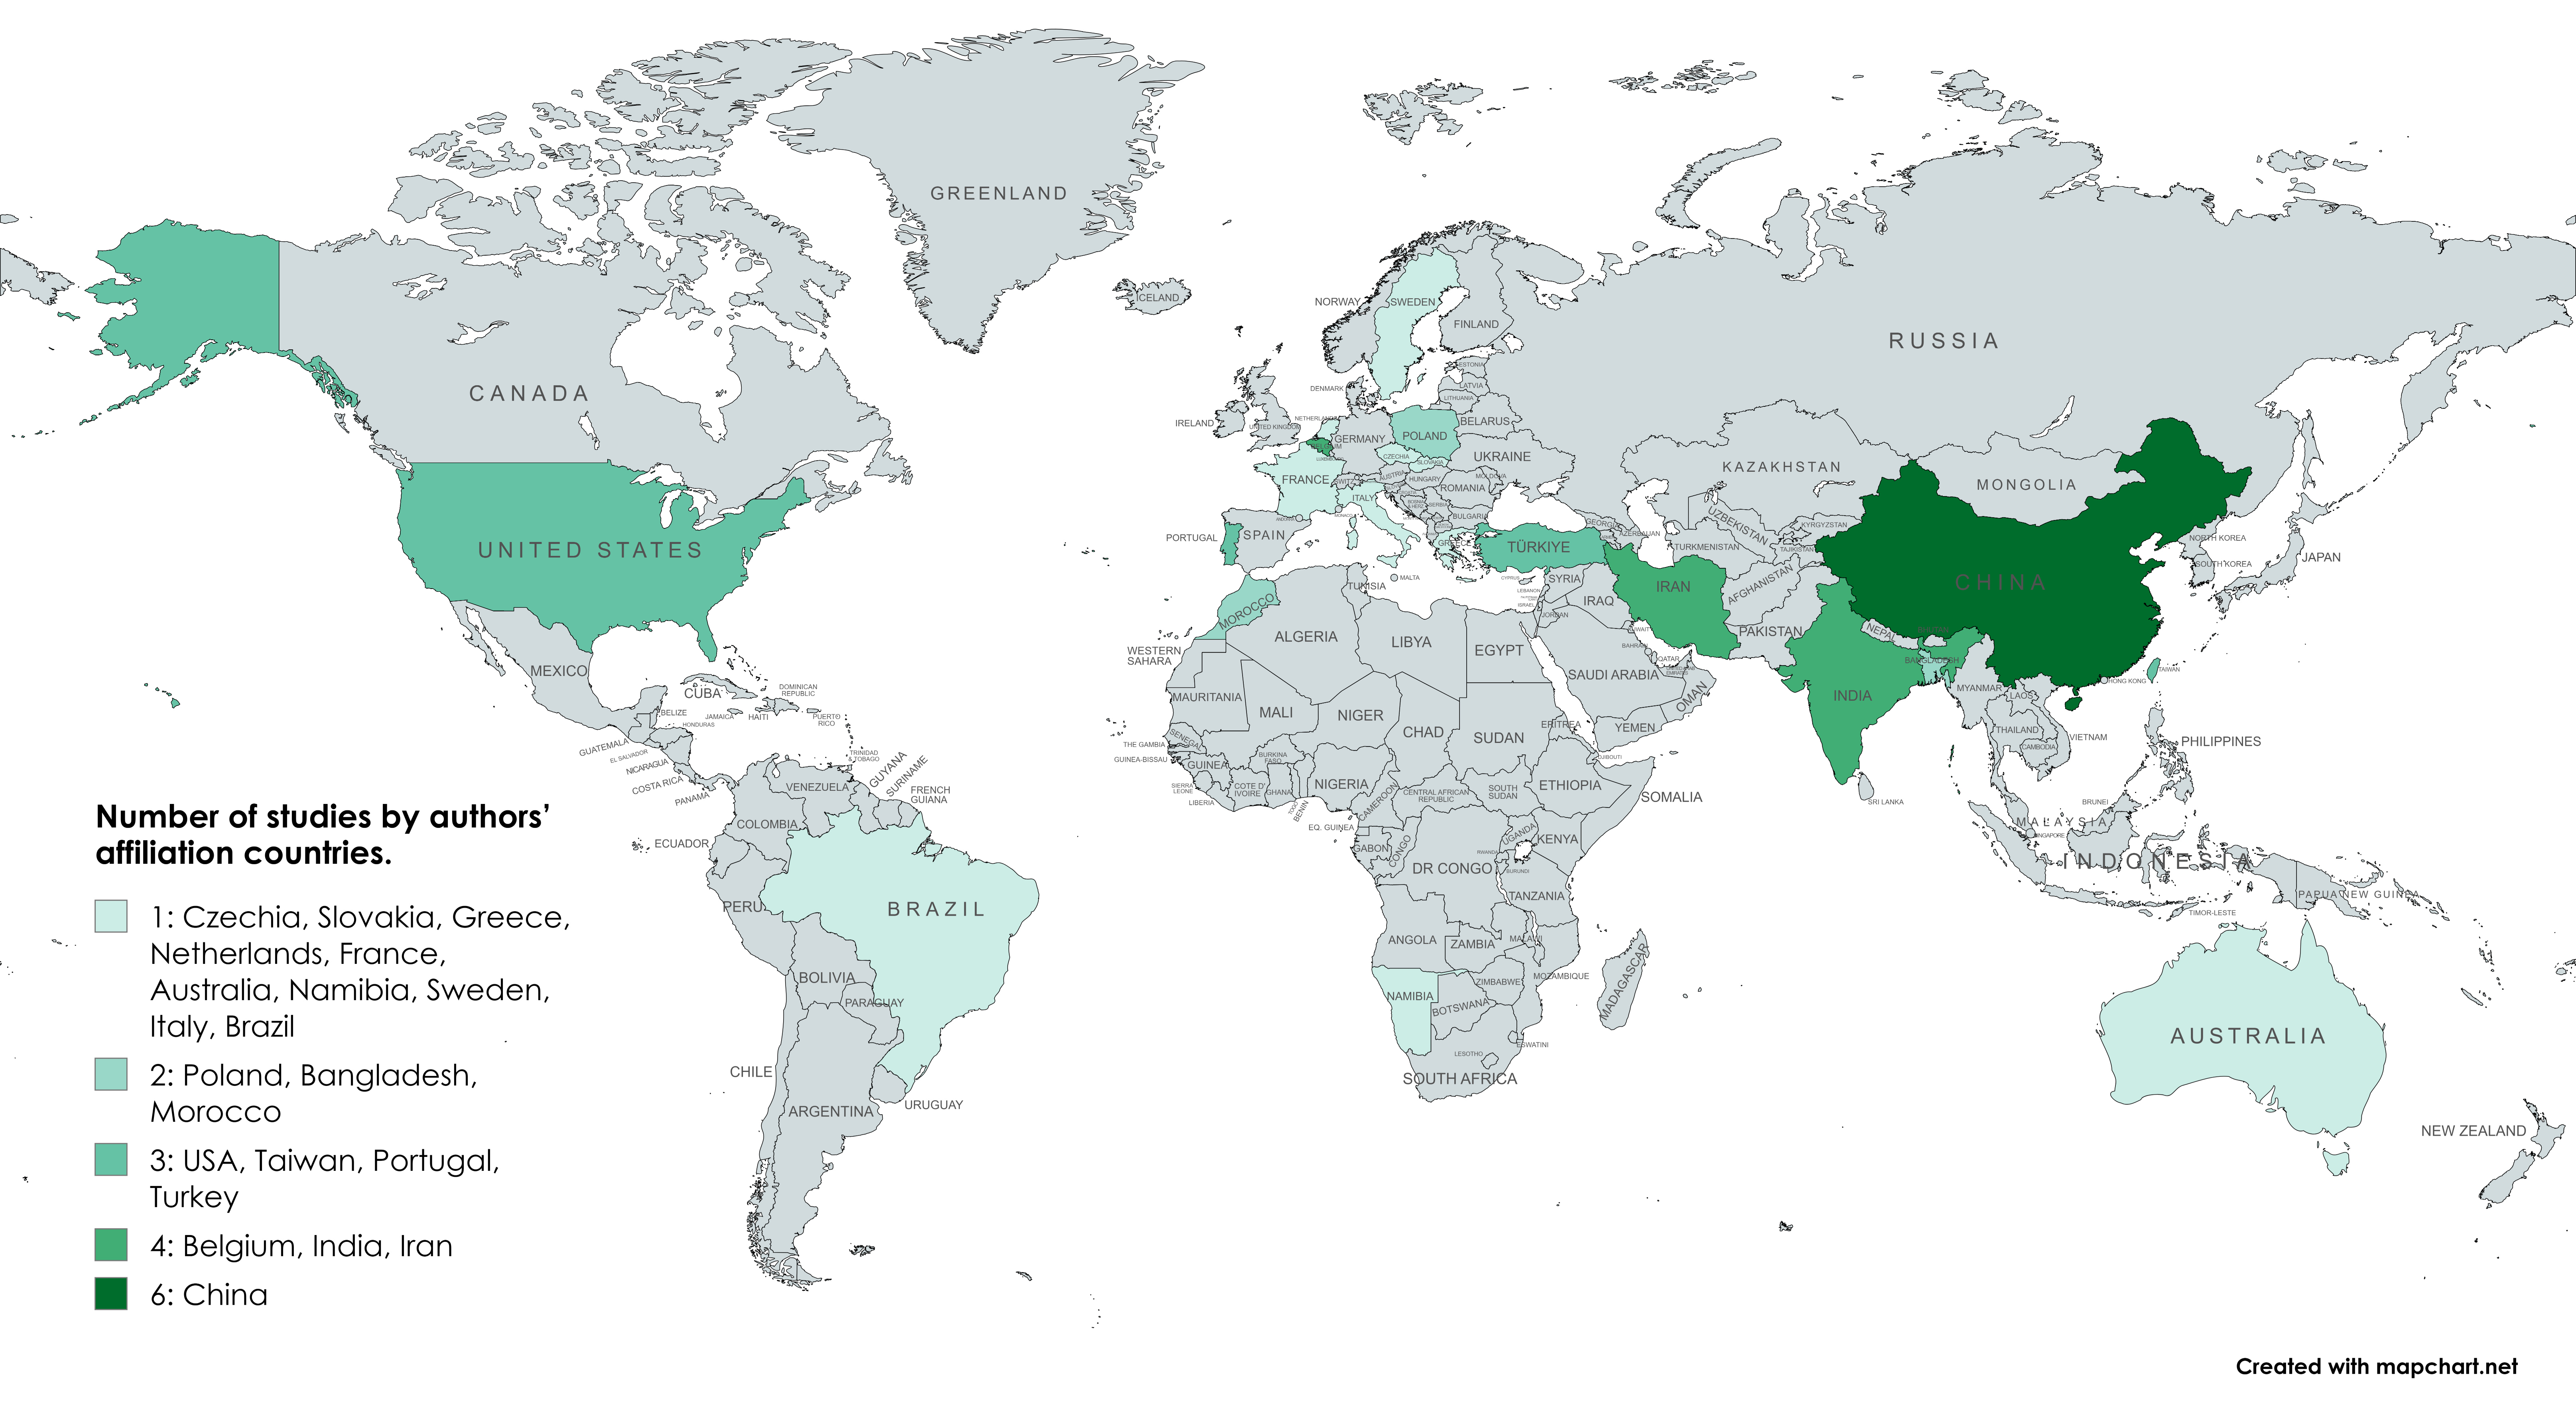
\includegraphics[width=\textwidth]{images/4_RESULTS/PS_RQ3_affiliation_countries.png}
    \caption{Distribution of selected studies by country of affiliation of authors.}
    \label{fig:PS_RQ3_Affiliation_Countries_Map}
\end{figure}    


 \textcolor{blue}{Figure \ref{fig:PS_RQ3_Affiliation_Countries_Map} presents the results of the author's affiliated country. Each country is counted only once per study, regardless of the number of authors affiliated with that country. If a study has authors from multiple countries, it is assigned to each of those countries. China had the highest representation, with six associated publications, followed by India, Belgium, and Iran, each contributing four publications. The United States, Taiwan, Portugal, and Turkey, each with three associated publications. Bangladesh, Morocco, and Poland contributed two publications each, while the remaining 10 countries were represented by a single publication.
It is worth noting that most publications originate from Asia, highlighting the region's particularly strong interest in the topic.}

\textcolor{orange}{Table \ref{tab:descriptive-summary} summarizes the main descriptive findings of the included studies.}

\begin{table}[H]
    \centering
    \caption{\textcolor{blue}{Summary of the main descriptive findings of the included studies}}
    \label{tab:descriptive-summary}
    \scriptsize
    \renewcommand{\arraystretch}{1.15}
    \begin{tabular}{|>{\raggedright\arraybackslash}p{0.18\textwidth}|>{\raggedright\arraybackslash}p{0.57\textwidth}|>{\raggedright\arraybackslash}p{0.17\textwidth}|}
        \hline
        \rowcolor{lightgray}
        \textbf{Topic} & \textbf{Finding} & \textbf{Reference} \\ \hline
        Publication trend & The earliest included study was published in 2005, and 31 of the 41 selected studies (76\%) were published from 2021 onward. & Table~\ref{table:biblometric_analysis} \\ \hline
        Venue type & Of the 41 selected studies, 28 were journal papers and 13 were conference papers. & Table~\ref{table:biblometric_analysis} \\ \hline
        Venue concentration & With the exception of four papers published in \textit{Expert Systems with Applications}, the remaining studies were distributed across distinct venues. & Table~\ref{table:biblometric_analysis} \\ \hline
        Research areas & Computer Science was the most represented research area (29 studies), followed by Engineering (19) and Mathematics, Physics, and Astronomy (11). & Table~\ref{table:biblometric_analysis} \\ \hline
        Geographic distribution & China had the highest representation with six associated publications, followed by India, Belgium, and Iran with four each. Most publications originated from Asia. & Figure~\ref{fig:PS_RQ3_Affiliation_Countries_Map} \\ \hline
    \end{tabular}
\end{table}


\begin{table}[H]
    \centering
    \caption{\textcolor{blue}{Bibliometrics of the included studies}}
    \label{table:biblometric_analysis}
    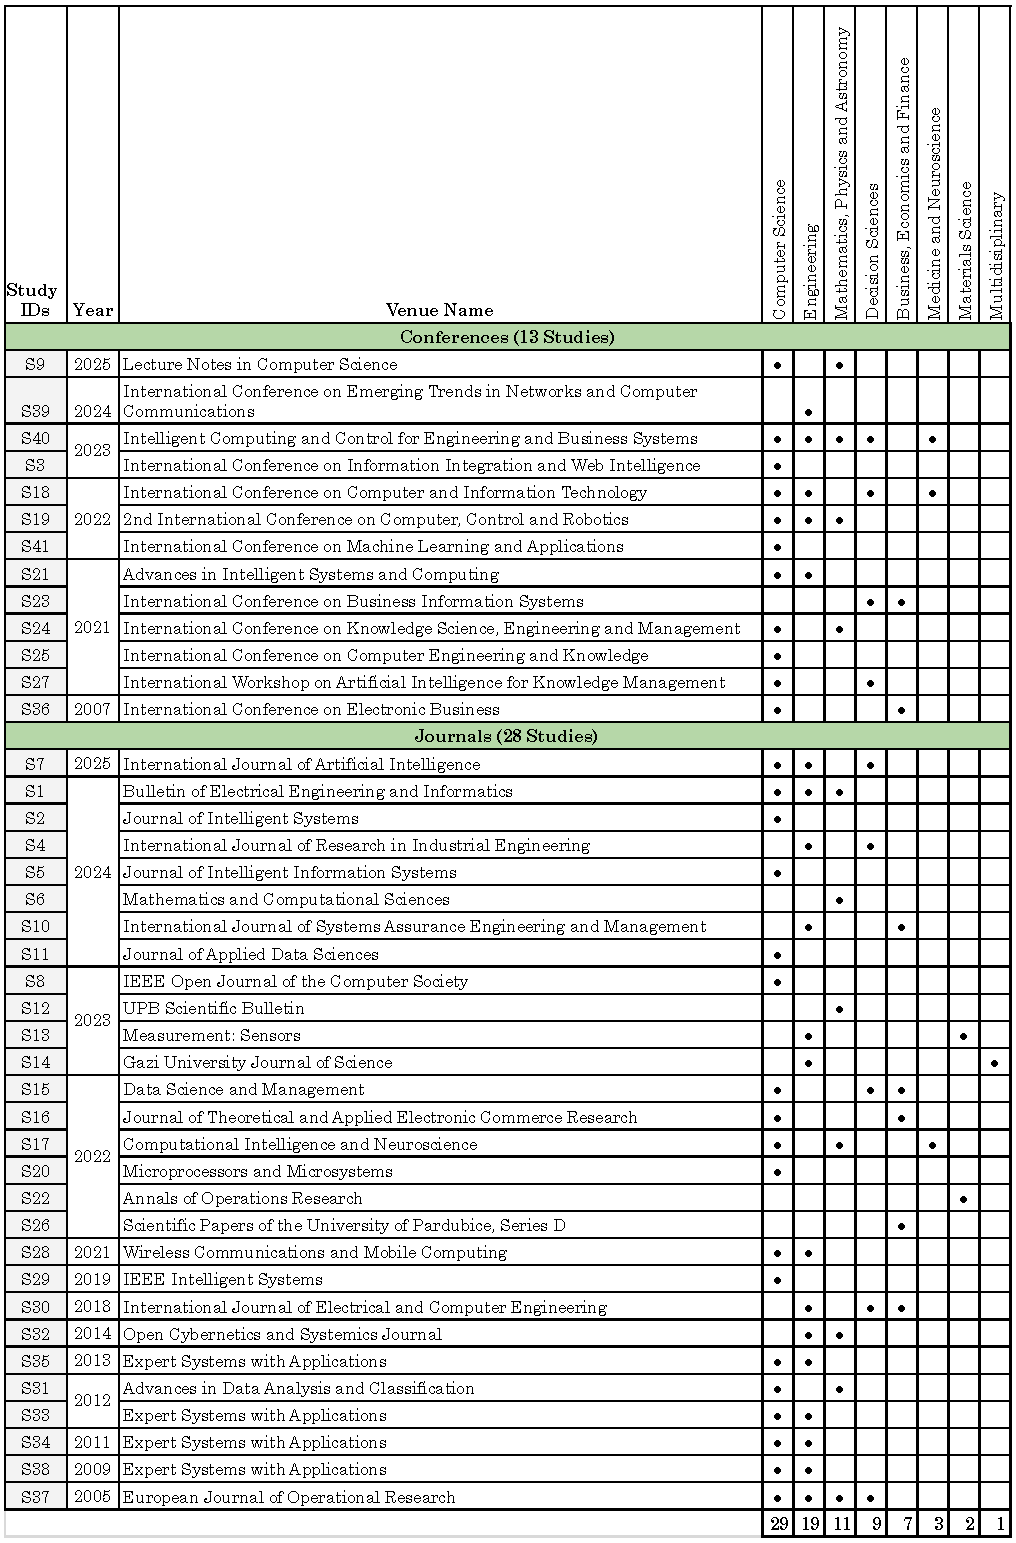
\includegraphics[width=0.91\textwidth]{pdf_tables/results/Bibliometrics_analysis.pdf}
\end{table}


\begin{comment}
\subsection{Answers to Publication Space Research Questions (PS-RQs)}
\subsubsection{\PSRQone}
%How are the selected studies distributed by publication year and venue type?

%proceed with the result and then insert the fact that there were no restrictions placed
No restrictions were applied to the publication date during the selection process of the primary studies. However, the earliest paper included in the analysis was published in 2005. As shown in Figure \ref{fig:PS_RQ1_venue_trend}, of the 41 selected papers, 31 (76\%) were published from 2021 onward, indicating a growing interest in this topic in recent years. It is important to note that the low number of papers for 2025 is due to the fact that the paper extraction was carried out at the end of January; therefore, only papers published before this date were included.
Among the 41 selected papers, 28 were published in journals, and 13 in conference proceedings (see Figure \ref{fig:PS_RQ1_pie_chart}). 
%Before applying the quality criteria, the distribution between journal and conference publications was more balanced. This shift suggests that journal publications were more likely to meet the quality standards employed in this study.
This distribution highlights a clear preference for journal publications, which may reflect their higher likelihood of meeting the quality standards employed in this study.

%TODO: Make the year of the graph more readable


\begin{figure}[h!]
    \centering
    \begin{subfigure}{0.48\textwidth}
        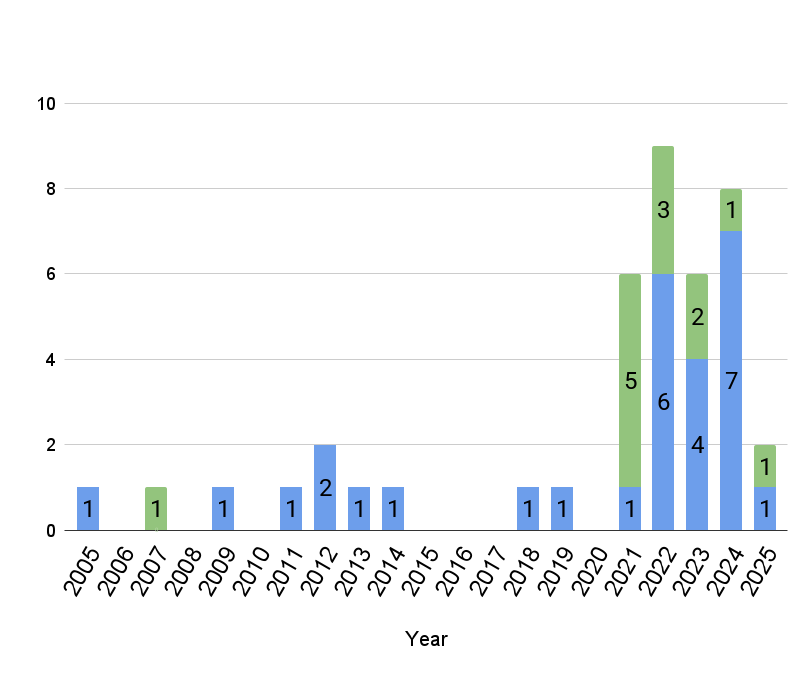
\includegraphics[width=\linewidth]{images/4_RESULTS/PS_RQ1_venue_trend.png}
        \caption{}
        \label{fig:PS_RQ1_venue_trend}
    \end{subfigure}   
    \hspace{0.02\textwidth}
    \begin{subfigure}{0.48\textwidth}
        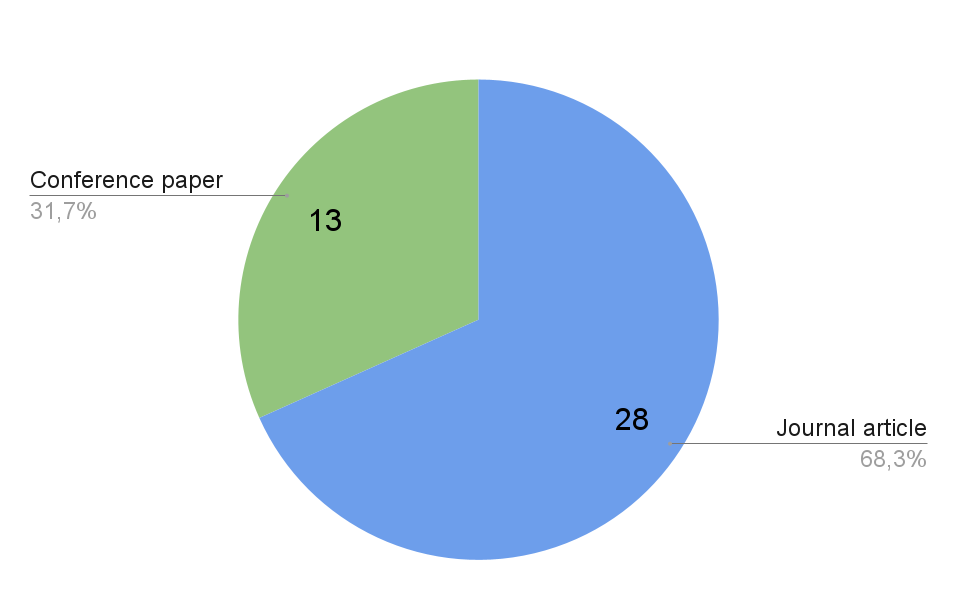
\includegraphics[width=\linewidth]{images/4_RESULTS/PS_RQ1_venue_pie_chart.png}
        \vspace{0.06\textwidth}
        \caption{}
        \label{fig:PS_RQ1_pie_chart}
    \end{subfigure}  
    \caption{Distribution of selected studies by publication year (a) and venue type (b).}
\end{figure}



\subsubsection{\PSRQtwo}

Table \ref{table:PS_RQ2_venues} presents the various publication venues of the 41 studies included in this analysis, along with the corresponding Study IDs for each venue. With the exception of four publications in the journal "Expert Systems with Application", the remaining 37 studies were each published in a distinct venue. Figure \ref{fig:PS_RQ2_research_area_distribution} illustrates the distribution of subject areas associated with the venues of all selected publications. 
As not all conferences provide publicly available information on their subject areas, a procedure was adopted to ensure consistency in the analysis. The areas of interest for journal articles were obtained from Scimago\footnote{\url{https://www.scimagojr.com}}. For conferences lacking this information, the corresponding subject areas were retrieved from Scopus\footnote{\url{https://www.scopus.com}}.

As expected for research on customer churn prediction using artificial intelligence, the dominant subject area associated with the publication venues of the selected studies was Computer Science with 29 studies, followed by Engineering with 19 studies, and subsequently by 'Mathematics, Physics, and Astronomy' with 11 studies. 'Business, Economics, and Finance' appeared in 7 studies, while Medicine and Neuroscience, Material Sciences, and the Multidisciplinary category were the least represented fields, with only 3, 2, and 1 associated studies, respectively. It is worth noting that each venue can be associated with multiple subject areas, meaning that the total number of subject-area associations exceeds the 41 selected studies.
%add numbers regarding the information provided (how many were on CS, etc) and provide the information first and then any comments (THIS IS VALID FOR ALL ANSWERS). (Done)

%Article -> Journal (Table) (Done)



\begin{table}[htbp]
\centering
\footnotesize
\renewcommand{\arraystretch}{1.1}
\caption{Study publication venues.}
\label{table:PS_RQ2_venues}
\resizebox{0.8\textwidth}{!}{
\begin{tabular}{|
  >{\raggedright\arraybackslash}m{12.5cm}
  |>{\centering\arraybackslash}m{2cm}|}
\hline
\rowcolor[HTML]{D5E8D4} 
\textbf{Venue Name} & \textbf{Study IDs} \\ \hline
\rowcolor{lightgray} 
\multicolumn{2}{|c|}{\textbf{Journals}} \\ \hline
Bulletin of Electrical Engineering and Informatics & S1 \\ \hline
Journal of Intelligent Systems & S2 \\ \hline
International Journal of Research in Industrial Engineering & S4 \\ \hline
Journal of Intelligent Information Systems & S5 \\ \hline
Mathematics and Computational Sciences & S6 \\ \hline
International Journal of Artificial Intelligence & S7 \\ \hline
IEEE Open Journal of the Computer Society & S8 \\ \hline
International Journal of Systems Assurance Engineering and Management & S10 \\ \hline
Journal of Applied Data Sciences & S11 \\ \hline
UPB Scientific Bulletin & S12 \\ \hline
Measurement: Sensors & S13 \\ \hline
Gazi University Journal of Science & S14 \\ \hline
Data Science and Management & S15 \\ \hline
Journal of Theoretical and Applied Electronic Commerce Research & S16 \\ \hline
Computational Intelligence and Neuroscience & S17 \\ \hline
Microprocessors and Microsystems & S20 \\ \hline
Annals of Operations Research & S22 \\ \hline
Scientific Papers of the University of Pardubice, Series D & S26 \\ \hline
Wireless Communications and Mobile Computing & S28\\ \hline
IEEE Intelligent Systems & S29 \\ \hline
International Journal of Electrical and Computer Engineering & S30 \\ \hline
Advances in Data Analysis and Classification & S31 \\ \hline
Open Cybernetics and Systemics Journal & S32 \\ \hline
Expert Systems with Applications & S33, S34, S35, S38 \\ \hline
European Journal of Operational Research & S37 \\ \hline
\rowcolor{lightgray} 
\multicolumn{2}{|c|}{\textbf{Conferences}} \\ \hline
International Conference on Information Integration and Web Intelligence & S3 \\ \hline
Lecture Notes in Computer Science & S9 \\ \hline
International Conference on Computer and Information Technology & S18 \\ \hline
International Conference on Computer, Control and Robotics & S19 \\ \hline
Advances in Intelligent Systems and Computing & S21 \\ \hline
International Conference on Business Information Systems & S23 \\ \hline
International Conference on Knowledge Science, Engineering and Management & S24 \\ \hline
International Conference on Computer Engineering and Knowledge & S25 \\ \hline
International Workshop on Artificial Intelligence for Knowledge Management & S27 \\ \hline
International Conference on Electronic Business & S36 \\ \hline
International Conference on Emerging Trends in Networks and Computer Communications & S39 \\ \hline
Intelligent Computing and Control for Engineering and Business Systems & S40 \\ \hline
International Conference on Machine Learning and Applications & S41 \\ \hline
\end{tabular}
}
\end{table} %now is left aligned




% Need to somehow reference the studies to they appear in the biblograpy 

\begin{figure}[h]
    \centering
    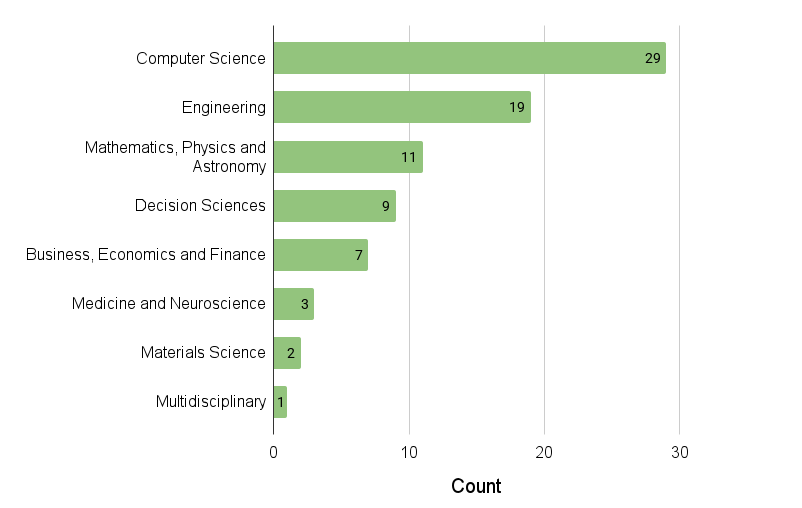
\includegraphics[width=0.8\textwidth]{images/4_RESULTS/PS_RQ2_research_area_distribution.png}
    \caption{Distribution of selected studies by research areas of the publication venues.}
    \label{fig:PS_RQ2_research_area_distribution}
\end{figure}  





\subsubsection{\PSRQthree}

%This section presents the affiliated countries for each publication. Each country is counted only once per study, regardless of the number of authors from that country. For example, if multiple authors in a single study are affiliated with the same country, it is counted as a single occurrence.

%Among the included studies, 12 were single-author publications, 36 studies had authors from the same country whereas 5 publications involved affiliations from two different countries. No study featured authors from more than two countries.



\end{comment}
%PRISMA Flowchart used for paper selection; Classification of each analyzed %paper; majority of Figures are added now.


\subsection{Answers to \textcolor{blue}{Research Questions (RQs)}}
%Tell about what we explain in this section. Give the definition, the number of papers that use it and why.


\subsubsection{\RSRQone}
\label{sec:RQ1}

In non-contractual settings such as Fast Moving Consumer Goods (FMCG) and e-commerce, defining churn presents a significant challenge. Unlike contractual industries, where customers formally terminate their relationship, churn in non-contractual sectors is a behavioral inference rather than a clearly observable event. Our review found that more than one-third of the 41 surveyed studies did not provide a clear definition of churn. In many cases, this omission was due to the use of pre-processed or third-party datasets, particularly those sourced from platforms such as Kaggle\footnote{\url{kaggle.com}}, where churn is provided as a pre-labeled flag with minimal or no documentation or behavioral context. Moreover, several studies relied on external datasets or cited sources that were either inaccessible or insufficiently described, rendering their churn definitions non-replicable. Even when a definition was provided, it was often vague or overly simplistic, lacking the detail necessary for methodological transparency and reproducibility.

%\begin{table}[H]
%    \centering
%    \caption{Churn Definition Groups.}
%    \label{fig:RS_RQ1_churn_definition}
%    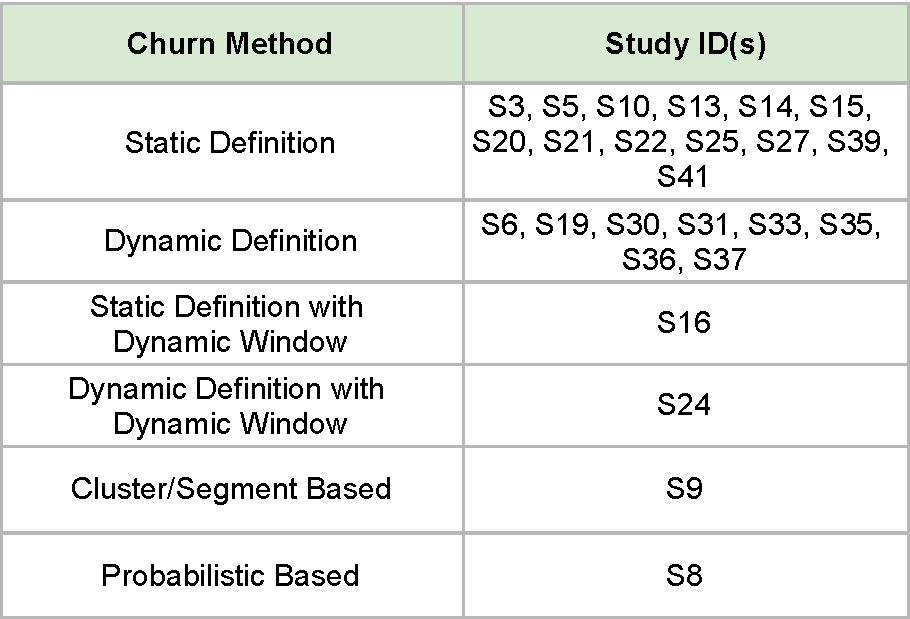
\includegraphics[width=.5\textwidth]{pdf_tables/results/RS_RQ1_churn_definition.pdf}
%\end{table}

\begin{table}[h]
    \caption{Adopted churn definitions and associated studies.}
    \label{tab:RS_RQ1_churn_definition}
    \centering
    %{\fontfamily{phv}\selectfont   % inizio gruppo → Helvetica/Arial-like
    \scriptsize                 % o \footnotesize, \small…
    \resizebox{0.7\textwidth}{!}{
    \begin{tabular}{|
  >{\centering\arraybackslash}m{4.5cm}
  |>{\centering\arraybackslash}m{5cm}|}
    \hline
    \rowcolor[HTML]{D5E8D4} 
    \rule[-1.5ex]{0pt}{4ex}\textbf{Churn definition}
  & \rule[-1.5ex]{0pt}{4ex}\textbf{Study ID(s)} \\ \hline
    Static & S3, S5, S10, S13, S14, S15, S20, S21, S22, S25, S27, S39, S41 \\ \hline
    Dynamic & S6, S19, S30, S31, S33, S35, S36, S37 \\ \hline
    Static with dynamic window & S16, S23 \\ \hline
    Dynamic with dynamic window & S24 \\ \hline
    Cluster/Segment based & S9 \\ \hline
    Probabilistic based & S8 \\ \hline
    \end{tabular}
    }
 % }% fine gruppo → torna al font normale qui
\end{table}


%We begin by describing the different categories as can be seen in Table \ref{tab:RS_RQ1_churn_definition} of churn prediction used in the selected studies.



\textcolor{blue}{To classify heterogeneous definitions in a consistent way, we conducted a thematic analysis of the churn definitions reported in the selected studies. To the best of our knowledge, no systematic typology of churn in non-contractual retail contexts exists.  Therefore, our analysis focuses on the operational definitions of churn used in practice rather than on new conceptual types of churn.
We used the data extraction form described in Section \ref{sec:methodology} to collect, for each study, the textual definition of churn and the details of its specifications.
We then iteratively coded each study along two main dimensions: \emph{i.} how the temporal window used to assess churn is defined (fixed length that is identical for all customers vs.\ implicitly or explicitly customer-specific), and \emph{ii.} how churn is determined within that window (fixed heuristic thresholds on inactivity or spending, behaviour-based thresholds relative to a reference period, or data-driven mechanisms such as clustering or probabilistic models). 
By systematically combining the values of these two dimensions and applying the resulting scheme to all 26 studies that provide an explicit operational definition of churn, we derived a data-driven taxonomy of six archetypal churn definitions. This taxonomy is summarized in Table~\ref{tab:RS_RQ1_churn_definition}, together with the associated Study IDs, and provides a unifying lens to map heterogeneous definitions found in the literature. Although it is grounded in our sample, the taxonomy is general enough to be used as a reference framework in future research on churn prediction in non-contractual retail environments.
The following categories of churn definitions were identified:}


\begin{itemize}
    \item \textit{Static definition}: This is the most common and straightforward approach. Churn is defined based on a fixed window period (e.g., 90 days, 3 months, or 1 year) during which the absence or reduction of customer activity is interpreted as churn. The threshold (e.g., no spending or a significant drop in purchases) is applied uniformly across all customers, regardless of their behavioral patterns. While this method is easy to implement and interpret, it lacks personalization and may overlook individual variations in engagement.
    
    \item \textit{Dynamic definition}: This method employs fixed-length observation and labeling windows (e.g., P1 = 3 months, P2 = 3 months). Churn is identified based on significant changes in customer behavior between these two periods. For example, a customer is labeled as churned if their loyalty in P2 declines sharply compared to their behavior during P1, or if their spending in P2 falls below a threshold that is behaviorally derived from P1. This approach captures behavioral shifts and partial churn more effectively than static definitions.
    
    \item \textit{Static definition with dynamic window}: 
    %Churn is assessed using a dynamic observation window defined by an event, such as the absence of subsequent purchases. However, the threshold for labeling churn within this window, for example using criteria like no further purchases or no activity beyond a predefined duration, remains fixed. This approach introduces some adaptability in identifying the observation period while preserving the simplicity of a static threshold.
    This approach evaluates churn based on an observation window whose start and/or length are dynamically determined by an event specific to the customer's purchase history (e.g., the customer's first or most recent transaction), while the threshold used to label churn (e.g., no purchases) remains static and uniformly applied to all customers.
    This approach introduces some adaptability in identifying the observation period while preserving the simplicity of a static threshold.
    
    \item \textit{Dynamic definition with dynamic window}: This is the most flexible and personalized approach. Both the observation window and the churn threshold are determined based on each customer’s unique behavioral history. For example, the window start point can be determined by their second last purchase and the dynamic recency threshold for churn can be determined for each customer as a multiple of their last two transactions.. This fully dynamic strategy enables highly tailored churn definitions and is commonly adopted in advanced models that prioritize precision over simplicity.

    \item \textit{Cluster/segment-based}: In this category, churn is inferred through data-driven segmentation techniques, such as K-means clustering, which group customers based on behavioral patterns. Customers assigned to groups exhibiting a complete absence or substantial reduction of activity are labeled as churners. This unsupervised approach does not rely on predefined thresholds, but rather identifies churn through emergent patterns in the data. Only one study employed this definition.
     
    \item \textit{Probabilistic-based}: This approach uses statistical or machine learning models to estimate the probability that a customer remains active. When this probability falls below a predefined threshold, the customer is classified as a churner. This method allows for dynamic adjustment based on differing consumption patterns and cycles. Among the reviewed studies, only one adopted this method.

\end{itemize}

%TODO: once this part is checked and the extraction is finalized, add a final sentence to state the level of the definitions provided


It is interesting to note that this simple approach dominates the literature with 13 studies using this method. This is followed by the dynamic definition method, which is utilized by 9 studies. The static definition with dynamic window approach is used by 2 studies. The other more bespoke approaches, including probabilistic and segmentation methods, are utilized only by one study.

\subsubsection{\RSRQtwo}
\label{sec:RQ2}
The analysis of the 41 selected studies revealed a wide range of features employed for customer churn prediction,  with some proving particularly effective in capturing churn-related behavior. Due to inconsistent terminology used across studies, feature names were standardized where possible to enable consistent comparison. When only intermediary or derived variables were reported, they were traced back and mapped to their most likely source features to align with a common feature taxonomy.

Variables such as \textit{Customer ID}, \textit{Transaction ID}, and other similar identifiers were excluded, as they do not provide meaningful information for churn prediction. These variables are primarily used within the data processing pipeline to consolidate records at the customer level.

The top section of Table \ref{table:RS_RQ2_features} lists the features used for churn prediction across the selected studies, indicating for each study whether they were used and, if applicable, whether they were identified as top features.
Empty circles (\textopenbullet) denote intermediary or derived variables, while filled circles (\textbullet) mark features explicitly identified as most important in the studies. Columns corresponding to studies with unclear source features are shaded in light grey.

%In cases where the available information was not sufficient to identify the original source features, the corresponding study row is shaded in light grey. When such information is available, the feature is indicated with an empty circle symbol (\textopenbullet). 
%If the study explicitly assessed the contribution of individual features to predictive performance, the best features identified by the study are then marked by a filled circle (\textbullet). 
The bottom section summarizes the use of feature categories. Each category is marked for a study if at least one variable from that category was included in the study. For studies in which the source features could not be fully identified but enough details were available to determine usage at the category level, only the relevant categories are indicated. These columns are also shaded in grey.
%We now describe the six feature categories identified, offering insights into each category. 

\textbf{\begin{table}[t]
    \centering
    \caption{Features used for churn prediction, with top-ranked features highlighted.
    %\DD{}{Consider highlighting in the table, e.g., with a round rectangle overlapping it, rows associated features common to most studies/datasets, and rows associated to best predicting features]}
    }
    \label{table:RS_RQ2_features}
    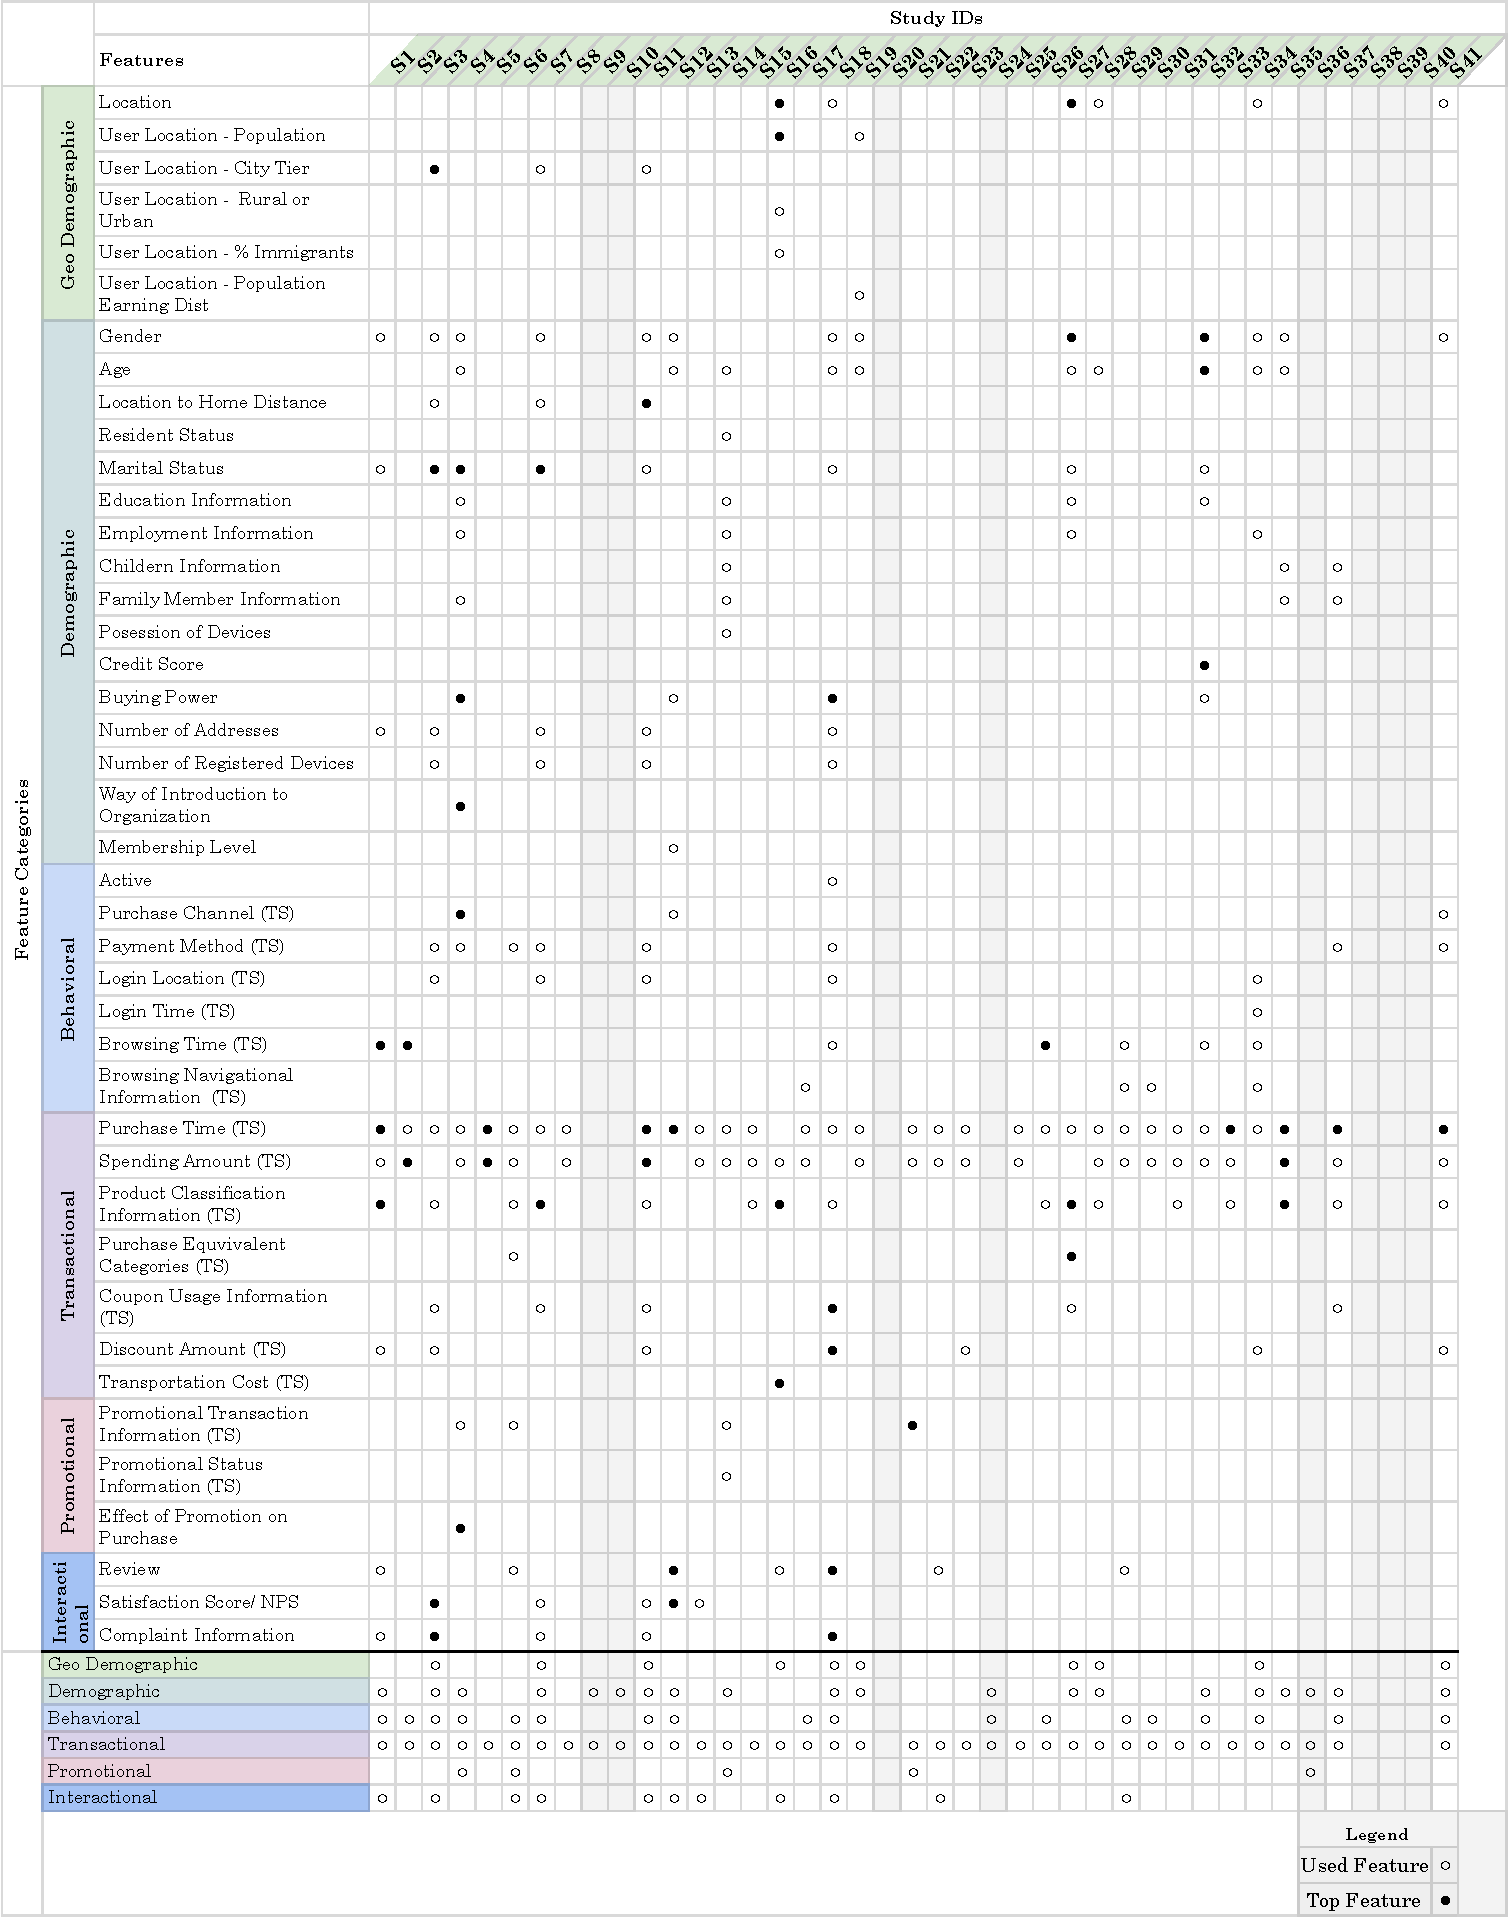
\includegraphics[width=\textwidth]{pdf_tables/results/RS_RQ2_features.pdf}
\end{table}}
\FloatBarrier

Subsequently, we present our observations regarding the specific features employed in the selected studies, with particular attention to those identified as most effective for churn prediction. 
%Overall, the features used can be broadly grouped into six main categories:


\begin{enumerate} 
\item \textit{Geo-demographic:}
Features belonging to this category capture the demographic characteristics of the customer's location (e.g., population density, income levels, economic activity, neighborhood composition), rather than the customer's personal attributes. %Examples include local population density, average income levels, regional economic activity, and neighborhood composition. 
While indirect, these features can provide useful contextual signals for customer behavior.

\item \textit{Demographic:}
This category includes personal demographic details of the customer, such as gender, age, marital status, occupation, and education level. These features are typically available early in the customer lifecycle and can aid in early-stage churn prediction.

\item \textit{Behavioral:}
Behavioral features capture how customers interact with the business outside of transactions. In e-commerce settings, this may include browsing history, visit frequency, time spent on product pages, and preferred channels (e.g., mobile vs. desktop). These features provide insight into customer engagement and interest before purchase decisions.

\item \textit{Transactional:}
This group includes features derived from customer transactions, such as purchase time, amount spent, and item category. These features are used to create aggregated (or engineered) features like purchase frequency, total spend, average basket size, recency of the last purchase, and product categories purchased. These are among the most widely used and influential churn predictors.

\item \textit{Promotional:}
Promotional features refer to both the historical promotional activity of the retailer (e.g., discount campaigns, coupons) and the customer's responsiveness to these promotions. These features may include the number of promotional items purchased, redemption rates, and purchase patterns during sales events.

\item \textit{Interactional:}
Interactional data arises when customers voluntarily engage with the company beyond purchases. This may include customer reviews, feedback surveys, satisfaction scores, support tickets, and complaints. These features offer qualitative insight into the customer experience and sentiment. 
\end{enumerate}

As shown in Table \ref{table:RS_RQ2_features}, most studies incorporate transactional features, particularly Purchase Time (TS) and Spending Amount (TS). This widespread usage can be attributed to the general availability of such data, as most retailers, whether operating online or with loyalty programmes in physical stores, routinely collect these variables. This widespread use highlights their value in predicting churn. 
%Furthermore, the consistent inclusion of these features suggests that the authors of the studies consider them to contain valuable information for predicting customer churn behavior. 
Many studies also use behavioral data, especially in e-commerce, where detailed web navigation logs complement transactional records, reflecting their predictive relevance. Customer profile attributes are also frequently used, indicating their potential value for churn modeling, though challenges in maintaining accurate and up-to-date profile data may impact its reliability in real-world applications.
%Another frequently used feature category relates to customer profile attributes. The regular use of this category suggests that researchers view such information as potentially informative for churn modeling. However, it is important to recognize that collecting and maintaining accurate and current profile data may be difficult in practice, which could affect its reliability in real-world applications.

The analysis of the selected studies revealed that top-ranked features are spread across various categories. This dispersion may result from different methodologies for evaluating feature importance, as varying techniques can yield different outcomes. The most informative features can also vary depending on the AI methods used, with more complex models potentially leveraging features more effectively. Additionally, feature engineering approaches influence how well features align with specific models, contributing to the variation observed in the ranking of top features.
%For the selected studies, an analysis of the trends among the most useful features reveals that the top-ranked feature in each case is not concentrated within a single category but is instead distributed across different feature groups. 
%This dispersion may be explained by the fact that each study employed a distinct methodology for evaluating feature importance, and different evaluation techniques can yield varying results. Additionally, the most informative features may vary depending on the AI method applied. For instance, a feature that contains a high amount of information may not be effectively leveraged by a simple machine learning model that lacks the complexity to extract its full predictive value. Feature usefulness can also be influenced by the specific feature engineering approaches employed. These techniques can shape how well a given feature aligns with a particular model. However, due to the wide range of methods used across the reviewed studies, such variations likely contribute to the observed variety in the relative ranking of top features. 

\subsubsection{\RSRQthree}
\label{sec:RQ3}
Feature engineering plays a crucial role in machine learning, as it can significantly enhance both model performance and interpretability. Of the 41 selected studies, 34 reported the use of some form of feature engineering. Below, we summarize the techniques employed, as illustrated in Table \ref{tab:PS_RQ_3_Feature_engineering_classification}.

\begin{table}[h]
    \caption{Classification of feature engineering techniques used in the reviewed studies.}
    \label{tab:PS_RQ_3_Feature_engineering_classification}
    \centering
    %{\fontfamily{phv}\selectfont   % inizio gruppo → Helvetica/Arial-like
    \scriptsize                 % o \footnotesize, \small…
    \resizebox{0.9\textwidth}{!}{
    \begin{tabular}{|
  >{\centering\arraybackslash}m{5cm}
  |>{\centering\arraybackslash}m{8cm}|}
    \hline
    \rowcolor[HTML]{D5E8D4} 
    \rule[-1.5ex]{0pt}{4ex}\textbf{Feature Engineering Method }
  & \rule[-1.5ex]{0pt}{4ex}\textbf{Study IDs} \\ \hline
    RFM and its extensions & S3, S5, S6, S9, S8, S17,
S21, S22, S28, S30, S31,
S33, S35, S36, S37, S41 \\ \hline
    Feature selection & S2, S4, S9, S12, S18, S21,
S19, S23, S27, S32, S35,
S38, S40 \\ \hline
    Feature transformation/
aggregation & S5, S9, S11, S15, S16,
S22, S23, S33, S35, S37 \\ \hline
    Customer segmentation
techniques & S19, S24, S27, S29, S30,
S37 \\ \hline
    Dimensionality reduction  & S9, S16, S19, S22, S23 \\ \hline
    \end{tabular}
    }
%  }% fine gruppo → torna al font normale qui    
\end{table}

\begin{itemize}
    \item \textit{RFM and its extensions}: This category includes studies that use Recency, Frequency, and Monetary (RFM) analysis or its extensions to evaluate customer behavior and value. These derived features are often used to create informative intermediate representations that aid in churn prediction. RFM-based techniques are the most commonly used feature engineering approach in the reviewed studies.
    
    \item \textit{Feature selection}: Studies in this category apply methods to identify the most relevant variables while eliminating redundant features.
    %A study is categorized under feature selection if it employs techniques to identify the most relevant variables in a dataset while eliminating redundant or less informative features. 
    This process enhances model robustness and reliability, while  reducing the computational cost of both training and inference. 
    
    \item \textit{Feature transformation and aggregation}: Studies in this category apply methods to modify, encode, or combine existing features to generate new, more informative representations. These transformations aim to create intermediate features that are more relevant for churn prediction than raw input data.
    %, thereby improving the learning process.

    \item \textit{Customer segmentation techniques}: This category includes studies applying clustering or segmentation strategies to group customers based on shared behaviors or characteristics. Segment information provides additional context, potentially improving churn prediction accuracy.
    %A study is included in this category if it applies clustering or segmentation strategies to group customers based on shared behaviors or characteristics. 
    %Incorporating segment information can provide additional context to the model, potentially improving churn prediction accuracy.

    \item \textit{Dimensionality reduction}: Studies that apply this method reduce the number of features by projecting data into a lower-dimensional space, while preserving essential information. Dimensionality reduction facilitates more efficient learning and decreases computational complexity.
\end{itemize}

As shown in Table \ref{tab:PS_RQ_3_Feature_engineering_classification}, RFM-based feature engineering techniques are the most commonly used, with 16 studies applying them, followed by feature selection methods (13 studies), feature transformation and aggregation (10 studies), customer segmentation (6 studies), and dimensionality reduction  (5 studies).

\subsubsection{\RSRQfour}
\label{sec:RQ4}
%AI Techniques for Churn Prediction
The reviewed literature shows a broad application of AI techniques to address customer churn prediction in the retail sector. These methods span from Artificial Neural Networks (ANNs), Convolutional Neural Networks (CNNs), and Long Short-Term Memory networks (LSTMs), to more traditional stochastic methods, including Naive Bayes and Poisson Processes, along with various other approaches.

Table~\ref{table:PS_RQ_4 Ai techniques table} summarizes the different AI techniques used by the reviewed studies. The symbols provide different information regarding the techniques' use: the empty circle define the method was used in the study (\scalebox{0.9}{\textopenbullet}); the filled circle indicate the best performing technique for the specific study (\scalebox{0.9}{\textbullet}); while the remaining symbol (\scalebox{0.6}{$\blacksquare$}) is used only if the technique was the only one used in the study.

Among the tree-based models, Random Forest, Gradient Boosting, and Decision Trees are the most widely adopted and effective techniques. Their strong performance can be attributed to their capacity to model non-linear relationships and interactions between variables, as well as their robustness to outliers and noise in data. Support Vector Machines (for the distance-based classifiers) are also commonly employed, and are often highlighted for being the top-performing models, probably due to their generalization ability. ANNs are widely used across multiple studies. These architectures excel in capturing complex patterns in sequential or high-dimensional data, which is particularly present in churn prediction situations where customer behavior evolves. In addition to these dominant categories, several studies also explore linear models like Logistic Regression, which, despite being one of the most explored, is seldom ranked as the most performing model.

Considered together, there is no clear evidence that suggests that a dominating model outperforms all others. The effectiveness of an AI technique appears to depend on the characteristics of the dataset, the balance of the classes, and the quality of feature engineering. That being said, tree-based models and neural networks consistently emerge as strong contenders, showing their versatility in modeling customer churn in the retail domain. More recent and advanced AI techniques, such as Transformer-based models, and deep learning, have yet to be widely explored or proven effective in the context of churn prediction within the retail sector.

\begin{table}[H]
    \centering
    \caption{AI techniques and their most effective applications across studies.
    %\DD{}{Consider highlighting in the table, e.g., with a border, rows associated to most employed AI techniques, and rows associated to AI techniques that resulted the best performing ones}
    }
    \label{table:PS_RQ_4 Ai techniques table}
    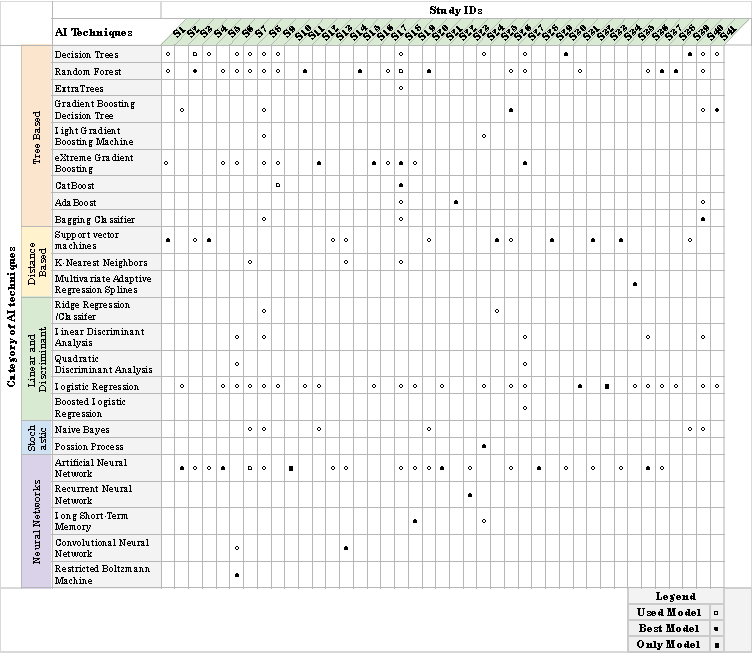
\includegraphics[width=\linewidth]{pdf_tables/results/RS_RQ4_techniques.pdf}
    %\vspace{-2.5cm}
\end{table}


\subsubsection{\RSRQfive}
\label{sec:RQ5}
Each application of AI typically requires a distinct set of evaluation metrics to effectively demonstrate and compare the performance of different algorithms, pre-processing methods, and training strategies. This is because the objectives and success criteria of AI tasks vary significantly between domains. A metric that may be highly informative in one context could be less meaningful or even misleading in another. This variability is particularly evident in churn prediction, where several specific factors influence metric selection. 
Our review of the 41 selected studies highlights these specific challenges. Firstly, churn datasets are often highly imbalanced, with churners representing only a small fraction of the total customer base. As a result, evaluation metrics that account for class imbalance are essential. Secondly, in practical business scenarios, marketing interventions aimed at reducing churn come at a cost. Therefore, it is often more critical to avoid misclassifying non-churners as churners (false positives) than to miss a few actual churners (false negatives). This cost-sensitive nature of churn prediction influences the choice and interpretation of performance metrics.

As shown in Table~\ref{table:metrics}, the most frequently used evaluation metrics across the selected studies include Accuracy, Precision, Recall, F1/F scores, and AUC-ROC. These metrics are particularly well-suited for assessing the performance of churn prediction algorithms. For example, Recall indicates the proportion of actual churners correctly identified by the model, while Precision reflects the proportion of predicted churners who are indeed true churners. These metrics are directly linked to the practical implications of false negatives and false positives, as discussed earlier. The F1 and F scores offer a harmonic mean of Precision and Recall, summarizing the model’s ability to balance these two aspects in a single value. In particular, the F score allows for adjustable weighting between Precision and Recall, providing flexibility to align the evaluation with specific business priorities. This makes it a valuable tool for deriving a single metric that captures both sensitivity and predictive accuracy. AUC-ROC is also widely used and regarded as a robust metric, especially in the context of class imbalance, which is common in churn prediction. It assesses the model’s ability to discriminate between churners and non-churners across all classification thresholds. In addition to these five commonly used metrics, several studies employ more specialized or domain-specific measures. These bespoke metrics are typically chosen to reflect particular research goals or business considerations of the authors.

\begin{table}[H]
    \centering
    \caption{Metrics to evaluate churn prediction techniques.}
    \label{table:metrics}
    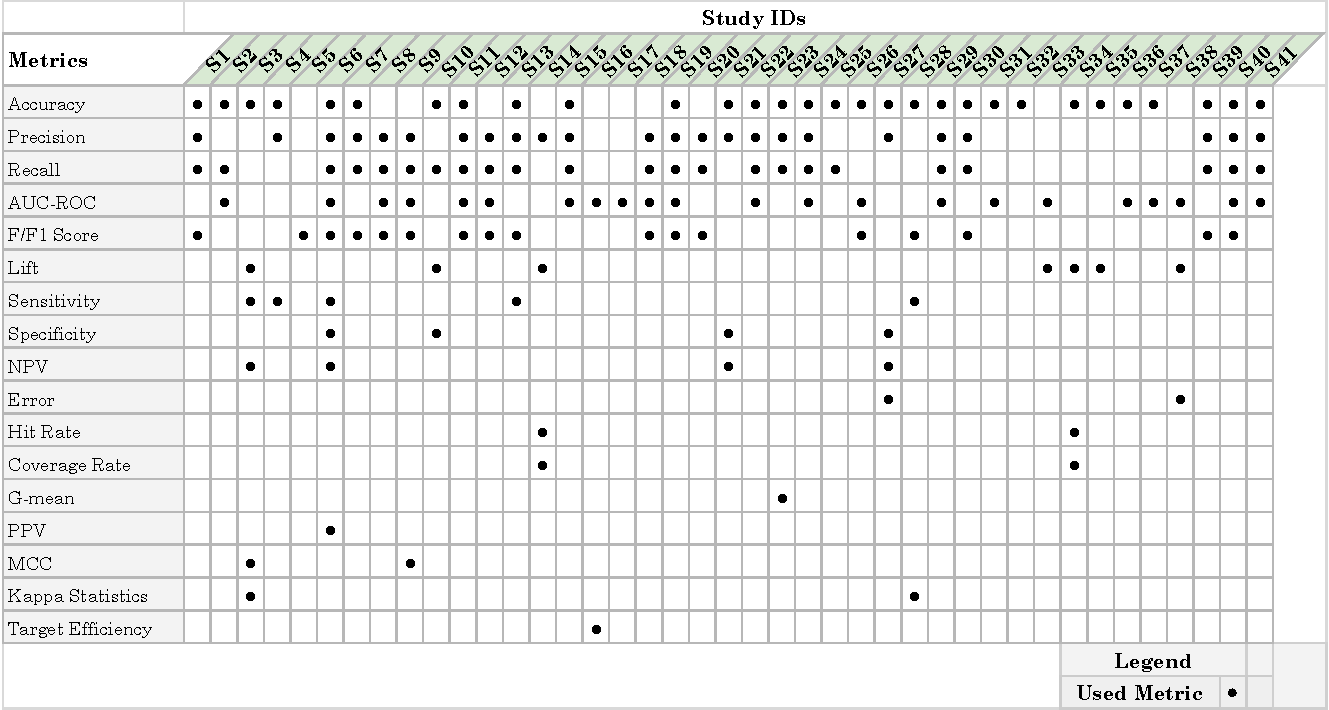
\includegraphics[width=\linewidth]{pdf_tables/results/RS_RQ5_metrics.pdf}
\end{table}


\subsubsection{\RSRQsix}
\label{sec:RQ6}
Very few papers provide a publicly available dataset (11 out of 41). However, it is still possible to find a diverse array of datasets employed for churn prediction in a non-contractual environment, having different contexts, data types, and business sectors. These datasets are primarily obtained from:
\begin{itemize}
    \item Open platforms such as Kaggle (e.g., the Retailrocket Recommender System Dataset \sid{D2} \cite{Dat2-verma2021ecommerce}, \sid{D4} \cite{Dat4-retailrocket2017dataset}, \sid{D5} \cite{Dat5-usmani2020pakistan}, \sid{D6} \cite{Dat6-regivm2021retail})
    \item Academic repositories (e.g., the Online Retail II dataset \sid{D3} \cite{Dat3-uci2021online}, \sid{D9} \cite{Dat9-recsyswiki2015grocery})
    \item Corporate contributions (e.g., the Brazilian E-Commerce Public Dataset by Olist \sid{D1} \cite{Dat1-olist2018brazilian}, \sid{D7} \cite{Dat7-dunnhumby2021source}, \sid{D8} \cite{Dat8-dunnhumby2021source})
\end{itemize}
\nocite{Dat1-olist2018brazilian, Dat2-verma2021ecommerce, Dat3-uci2021online, Dat4-retailrocket2017dataset, Dat5-usmani2020pakistan, Dat6-regivm2021retail, Dat7-dunnhumby2021source, Dat8-dunnhumby2021source, Dat9-recsyswiki2015grocery}

As illustrated in Table~\ref{table:available_datasets}, the datasets cover both online (E-Commerce) and offline (Brick-and-Mortar) scenarios and span multiple retail sectors, including merchandise, fashion, electronics, and food. These datasets differ not only in the retail sector they are related to, but also in structural characteristics, going from using only transactional records to multidimensional data including geo-demographic, behavioral, and interactional features. \\
It is interesting to note that the majority of the datasets are real-world datasets, but there is also a single synthetic dataset (i.e., the Retail Transaction Data) that is also used, showing attempts to simulate realistic churn behaviors for research purposes when actual data is limited or confidential. 

% DISCUSSION TOPIC? These synthetic datasets could be particularly useful for controlled experimentation and benchmarking if big and complex enough.
%is the following also a DISCUSSION TOPIC?
This research question clearly uncovered the difficulties associated with the churn prediction task: each business, sector, dataset, and even study set a different definition for churn (as seen in Section \ref{sec:RQ1}). This inherent feature of this problem creates difficulty in comparing frameworks (needing to be equal in not only the dataset, but also the churn definition), making it impossible in this review to make any kind of comparison.

The datasets that already provide a churn flag, stating whether the customer has churned or not, show insufficient documentation, i.e., it is impossible to trace back what the adopted definition of churn is. This impacts reproducibility and points to the need for greater transparency and standardization in data reporting. 
This review encourages the creation of a clear dataset description and the use of practices that can help future researchers better assess, compare, and build robust churn prediction models in the retail domain.

\begin{table}[h!]
\centering
\caption{Available datasets.}
\label{table:available_datasets}
%{\fontfamily{phv}\selectfont   % inizio gruppo → Helvetica/Arial-like
    \tiny                 % o \footnotesize, \small…
\resizebox{1\textwidth}{!}{
\begin{tabular}{
  |>{\centering\arraybackslash}p{0.1cm}
  |>{\centering\arraybackslash}p{1.8cm}
  |>{\centering\arraybackslash}p{0.7cm}
  |>{\centering\arraybackslash}p{1.3cm}
  |>{\centering\arraybackslash}p{1.3cm}
  |>{\centering\arraybackslash}p{1.1cm}
  |>{\centering\arraybackslash}p{2cm}
  |>{\centering\arraybackslash}p{1.8cm}
  |>{\centering\arraybackslash}p{0.7cm}
  |>{\centering\arraybackslash}p{0.7cm}
  |>{\centering\arraybackslash}p{0.7cm}
  |}
\hline
\rowcolor[HTML]{D9EAD3} 
      \multicolumn{1}{|c|}{\textbf{ID}}
      & \textbf{Dataset name}
      & \textbf{\begin{tabular}[c]{@{}c@{}}Pub.\\year\end{tabular}}
      & \textbf{\begin{tabular}[c]{@{}c@{}}Retail\\sector\end{tabular}}
      & \textbf{\begin{tabular}[c]{@{}c@{}}Synthetic/\\Real\end{tabular}}
      & \textbf{\begin{tabular}[c]{@{}c@{}}Online/\\Physical\end{tabular}}
      & \textbf{\begin{tabular}[c]{@{}c@{}}Features\\categories\end{tabular}}
      & \textbf{\begin{tabular}[c]{@{}c@{}}Dataset\\size\end{tabular}}
      & \textbf{\begin{tabular}[c]{@{}c@{}}Churn\\Flag\end{tabular}}
      & \textbf{\begin{tabular}[c]{@{}c@{}}Churn\\Rate\end{tabular}}
      & \textbf{\begin{tabular}[c]{@{}c@{}}Study\\IDs\end{tabular}}\\ \hline
\multicolumn{1}{|c|}{\sid{D1}} & \begin{tabular}[c]{@{}c@{}}Brazilian \\ e-commerce \\ public dataset \\ by Olist \\ \cite{Dat1-olist2018brazilian}\end{tabular} & 2018 & \begin{tabular}[c]{@{}c@{}}fashion, \\ mobile, \\ electronics, \\ appliance, \\ etc.\end{tabular} & Real & Online & Transactional & \# Orders: 100k & F & NA & \begin{tabular}[c]{@{}c@{}}S3,\\ S5,\\S10,\\ S20\end{tabular} \\ \hline
\sid{D2} & \begin{tabular}[c]{@{}c@{}}E-commerce \\ customer \\ churn analysis \\ and prediction \\ \cite{Dat2-verma2021ecommerce}\end{tabular} & 2021 & NA & NA & Online & \begin{tabular}[c]{@{}c@{}}Geodemographic, \\ Demographic,\\ Behavioural,\\ Transactional,\\ Interactional\end{tabular} & \# Rows: 5630 & T & 20.24\% & S7 \\ \hline
\sid{D3} & Online Retail II \cite{Dat3-uci2021online}& 2012 & gift-ware & Real & Online & Transactional & \begin{tabular}[c]{@{}c@{}}\# Instances: \\ 1,067M\end{tabular} & F & NA & S5, S8 \\ \hline
\sid{D4} & \begin{tabular}[c]{@{}c@{}}Retailrocket \\ recommender\\  system dataset \\ \cite{Dat4-retailrocket2017dataset}\end{tabular} & 2022 & \begin{tabular}[c]{@{}c@{}}fashion, \\ mobile, \\ electronics, \\ appliance, \\ etc\end{tabular} & Real & Online & \begin{tabular}[c]{@{}c@{}}Behavioural, \\ Transactional\end{tabular} & \begin{tabular}[c]{@{}c@{}}\# Events: 2,7M\\ \# Unique \\ Visitors: 1,4M\\ \# Product \\ Information: \\ 20M\\ \# Unique Items: \\ 417k\end{tabular} & F & NA & S26, S29 \\ \hline
\sid{D5} & \begin{tabular}[c]{@{}c@{}}Pakistan's \\ largest \\ e-commerce \\ dataset \\ \cite{Dat5-usmani2020pakistan}\end{tabular} & \begin{tabular}[c]{@{}c@{}}2020/\\ 2021\end{tabular} & \begin{tabular}[c]{@{}c@{}}fashion, \\ mobile, \\ electronics, \\ appliance, \\ etc.\end{tabular} & Real & Online & Transactional & \begin{tabular}[c]{@{}c@{}}\# Transactions: \\ 500K\end{tabular} & F & NA & S8 \\ \hline
\sid{D6} & \begin{tabular}[c]{@{}c@{}}Retail \\ Transaction \\ Data \\ \cite{Dat6-regivm2021retail}\end{tabular} & \begin{tabular}[c]{@{}c@{}}2017/\\ 2018\end{tabular} & NA & Synthetic & NA & Transactional & \begin{tabular}[c]{@{}c@{}}\# Transactions: \\ 125K\end{tabular} & F & NA & S25 \\ \hline
\sid{D7} & Carbo-loading \cite{Dat7-dunnhumby2021source} & \begin{tabular}[c]{@{}c@{}}Last \\ update: \\ 2023\end{tabular} & Food & Real & \begin{tabular}[c]{@{}c@{}}Offline \\ (Brick and \\ Mortar)\end{tabular} & NA & \begin{tabular}[c]{@{}c@{}}\# Transactions: \\ 5M+\end{tabular} & F & NA & S24 \\ \hline
\sid{D8} & \begin{tabular}[c]{@{}c@{}}The complete \\ journey \\ \cite{Dat8-dunnhumby2021source} \end{tabular} & NA & Food & Real & \begin{tabular}[c]{@{}c@{}}Offline \\ (Brick and \\ Mortar)\end{tabular} & NA & \begin{tabular}[c]{@{}c@{}}\# Transactions: \\ 10M+\end{tabular} & F & NA & S24 \\ \hline
\sid{D9} & A-feng dataset \cite{Dat9-recsyswiki2015grocery} & \begin{tabular}[c]{@{}c@{}}Last\\ update: \\ 2015\end{tabular} & Food & Real & \begin{tabular}[c]{@{}c@{}}Offline \\ (Brick and \\ Mortar)\end{tabular} & \begin{tabular}[c]{@{}c@{}}Geodemographic, \\ Demographic, \\ Transactional\end{tabular} & \begin{tabular}[c]{@{}c@{}}\# Transactions: \\ 817K\\ \# Users: 32k\\ \# Items: 23,8K\end{tabular} & NA & NA & S28 \\ \hline
\end{tabular}
}
%  }% fine gruppo → torna al font normale qui
\end{table}
\FloatBarrier

\subsubsection{\RSRQseven}
\label{sec:RQ7}
%\DD{}{A list of citations is followed by a period or comma, not the other way around. Correct.}

Fifteen of the 41 selected studies explicitly discuss challenges and limitations encountered in their research. These can be broadly categorized into five groups, as shown in Table \ref{tab:PS_RQ_7_Challenges_and_limitations}. A detailed description of the categories is provided below.


\begin{itemize}
    \item \textit{Data availability:} Datasets used to experiment with methods for customer churn prediction are often limited in size, synthetic, or come from a single retailer or business sector. Incorporating data from multiple sectors and/or retailers could help build more resilient models and uncover deeper behavioral patterns.

    \item \textit{Domain limitation:} This issue is closely linked to data availability and highlights the lack of data sources from diverse business domains. Much of the research on customer churn prediction is focused exclusively on either online or offline retail contexts, making it difficult to transfer findings or techniques across channels. Since customer dynamics can vary significantly across sectors, a domain-independent model needs to be trained on data with sufficient domain diversity to ensure generalizability.

    \item \textit{Lack of comparative frameworks:} This issue emphasizes the absence of comprehensive testing and comparisons across a broad spectrum of AI frameworks and techniques. Without such comparisons, it is difficult to draw reliable conclusions regarding the relative performance of different approaches for churn prediction.

    \item \textit{Computational resource limitation:} This issue pertains to constraints in computational resources available to researchers. Limited computational power prevents the exploration of optimal hyper-parameter configurations and restricts the ability to test larger or more complex models on substantial datasets, potentially limiting the performance and scalability of the proposed techniques.

    \item \textit{Lack of robustness:} This issue concerns instances where technical inconsistencies arise, such as results that contradict the researchers’ hypotheses or the presence of known weaknesses in the employed models that may introduce bias or skew results, undermining their theoretical validity.
\end{itemize}

\begin{table}[h]
\caption{Challenges and limitations presented in the reviewed studies.}
\label{tab:PS_RQ_7_Challenges_and_limitations}
\centering
\scriptsize
\resizebox{0.9\textwidth}{!}{
\begin{tabular}{|
>{\centering\arraybackslash}m{5cm}
|>{\centering\arraybackslash}m{8cm}|}
\hline
\rowcolor[HTML]{D5E8D4}
\rule[-1.5ex]{0pt}{4ex}\textbf{Challenges and Limitations}
& \rule[-1.5ex]{0pt}{4ex}\textbf{Study IDs} \\ \hline
Data availability & S4, S16, S21, S28, S31, S36, S37, S38 \\ \hline
Domain limitation & S4, S15, S29, S30, S31, S33, S37 \\ \hline
Lack of comparative frameworks & S16, S22, S23, S30 \\ \hline
Computational resource limitation & S15, S22 \\ \hline
Lack of robustness & S9, S38  \\ \hline
\end{tabular}
}
\end{table}


\begin{comment}
%Out of the 41 studies selected, 15 explicitly discussed the challenges faced in their research. 
The most prominent concern raised by the selected studies is data availability: datasets are often limited in size, synthetic, or come from a single retailer or sector. Incorporating data from multiple sectors and/or retailers could help build more resilient models and uncover deeper behavioral patterns \cite{S4-ID40-Barzegar, S16-ID325-Matuszelanski, S19-ID363-Agbemadon, S20-ID379-Baghla, S21-ID389-Seymen, S30-ID647-Rachid, S31-ID717-Migueis, S33-ID742-Migueis, S36-ID806-Ching, S37-ID826-Buckinx}.

Another challenge raised by the studies is linked to domain limitations. It is pointed out that much of the research on customer churn prediction is focused exclusively on either online or offline retail contexts, making it difficult to transfer findings or techniques across channels \cite{S4-ID40-Barzegar, S16-ID325-Matuszelanski, S30-ID647-Rachid, S31-ID717-Migueis, S33-ID742-Migueis, S37-ID826-Buckinx}.

The narrow model diversity is also pointed out by the authors, where they highlight that most works rely on a limited set of algorithms, often lacking in comparative analysis with more recent or diverse AI techniques. This lack of methodological breadth can make it harder to identify the best-performing approaches \cite{S16-ID325-Matuszelanski, S22-ID394-Wu, S30-ID647-Rachid}.

Some studies also point out that the computational costs are a common performance bottleneck. Processes such as grid search for hyperparameter tuning are rarely performed exhaustively, which may prevent models from reaching their optimal performance. The studies have cited the computational constraints as a reason behind not being able to fully explore the parameter space \cite{S15-ID297-Georgiou, S22-ID394-Wu, S38-ID833-Burez, S29-ID538-Berger}.
Therefore, when comparing different techniques, the observed performance may not reflect each method's full potential.
%, as resource constraints can limit the ability to optimize hyper-parameters effectively for each method.
Another limitation raised is related to the methodological assumptions and experimental design. For instance, some clustering approaches failed to meet variance assumptions, undermining their theoretical validity. In several cases, a lack of rigorous evaluation protocols was reported, raising questions about the robustness and reproducibility of the findings \cite{S9-ID95-Coolwijk, S23-ID396-Pondel, S38-ID833-Burez}.
\end{comment}

\subsubsection{\RSRQeight}
\label{sec:RQ8}
Of the 41 selected studies, 31 provided directions for future research. The proposed directions can be broadly grouped into seven categories which can be observed in Table \ref{tab:PS_RQ_8_Future_directions}. The details of the categories are as follows:

\begin{itemize}

    \item \textit{Exploring new frameworks:} Studies in this category suggest employing a broader range of AI techniques and fully exploiting these methods through hyperparameter tuning and architectural optimizations. The utilization of more advanced architectures, such as Recurrent Neural Networks, ensemble learning, transformers, and hybrid models combining supervised and unsupervised techniques, is expected to better capture sequential dependencies, rare events, and subtle patterns in customer behavior, potentially improving churn prediction performance. Additionally, to fully exploit the capabilities of AI models, studies propose optimization efforts, including hyperparameter tuning and dynamic adaptation to concept drift, which is gaining increasing attention. Techniques such as online learning, adaptive algorithms, and automated feature engineering pipelines are suggested to better handle evolving customer behaviors and seasonal trends.


    \item \textit{Data and domain augmentation:} Studies in this category propose integrating richer and more diverse data sources, including social media sentiment, transactional history, weather patterns, spatial data, and socio-economic indicators. Together, these sources can offer a more holistic view of customer behavior and improve the generalizability of predictive models across various contexts. Furthermore, incorporating data from different retail sectors, such as fashion, electronics, and others, can enhance generalizability by ensuring that datasets capture a wider range of customer behaviors, which often vary between domains.
    
    \item \textit{Customer segmentation and behavioral features:} Proposals in this category are similar to data augmentation efforts but focus specifically on incorporating behavioral features, such as web navigational data from e-commerce or hybrid retailers. Furthermore, some studies propose deriving intermediate features, such as customer segments, and providing this information to AI models to offer additional context about customers.
    
    \item \textit{Temporal dynamics:} Studies in this category propose techniques aimed at more effectively capturing and leveraging the temporal dynamics of data. Such proposals include utilizing time series data directly, as well as exploring methods that allow models to better capture time-based patterns, such as experimenting with different window lengths and time series scales.
    

    \item \textit{Explainability:} Studies propose techniques to improve the interpretability of AI models. This includes understanding the relative importance of various features by using tools such as Shapley values. Improving AI model explainability can foster greater trust in the models and provide deeper insights into the complex reasons behind customer churn.

    \item \textit{ROI impact:} Studies emphasize considering the return on investment (ROI) implications when evaluating churn prediction models. For example, falsely predicting a non-churner as a churner has a higher negative financial impact than failing to identify a potential churner, as promotional resources would be wasted in the former case.
    
    \item \textit{Real-world deployment:} Studies propose validating customer churn prediction models in real-world environments. Such validation would not only help assess churn prediction performance but also reveal the actual financial impact on businesses when these systems are integrated into promotional campaigns.
    
\end{itemize}

\begin{table}[H]
\caption{Future directions presented in the reviewed studies.}
\label{tab:PS_RQ_8_Future_directions}
\centering
\scriptsize
\resizebox{0.9\textwidth}{!}{
\begin{tabular}{|
>{\centering\arraybackslash}m{5cm}
|>{\centering\arraybackslash}m{8cm}|}
\hline
\rowcolor[HTML]{D5E8D4}
\rule[-1.5ex]{0pt}{4ex}\textbf{Future directions}
& \rule[-1.5ex]{0pt}{4ex}\textbf{Study IDs} \\ \hline
Exploring new frameworks & S3, S4, S5, S6, S7, S9, S10, S11, S13, S14, S18, S19, S20, S22, S23, S24, S25, S26, S28, S30, S33, S38, S41 \\ \hline
Data \& domain augmentation & S2, S3, S4, S7, S10, S11, S16, S19, S20, S21, S22, S26, S30, S31, S33, S36, S37 \\ \hline
Customer segmentation and behavioral features & S6, S14, S15, S16, S21, S22, S28, S30, S33 \\ \hline
Temporal dynamics & S4, S5, S15, S21, S23, S24, S31, S36 \\ \hline
Explainability & S5, S7, S26, S41  \\ \hline
ROI impact & S3, S12, S15, S37 \\ \hline
Real-world deployment & S2, S14 \\ \hline
\end{tabular}
}
\end{table}

%Approximately three quarters of the selected studies offered insights into future research directions, revealing a growing consensus on how to improve customer churn prediction using AI techniques. 
\begin{comment}
    
Several of the 41 studies analyzed propose future research directions, revealing a growing consensus on how to improve Customer Churn Prediction using AI techniques. One key area involves the integration of richer and more diverse data sources, including social media sentiment, transactional history, weather patterns, spatial data, and socio-economic indicators, which together can offer a more holistic view of customer behavior and improve the generalizability of predictive models across contexts \cite{S3-ID223-Beckhauser,S11-D105-Sunarya,S16-ID325-Matuszelanski,S19-ID363-Agbemadon}.

Another promising direction is the improvement of feature engineering and segmentation strategies, through techniques such as signal transformation, wrapper selection, or behavioral clustering. These methods extract meaningful patterns from complex datasets, particularly regarding temporal dynamics or customer lifecycle transitions \cite{S3-ID223-Beckhauser,S9-ID95-Coolwijk,S15-ID297-Georgiou,S21-ID389-Seymen,S23-ID396-Pondel}.

Researchers also highlight the need for developing explainable AI models, particularly deep learning architectures that incorporate intrinsic attention mechanisms or Shapley interpretability tools. This could improve both stakeholder trust and diagnostic capabilities in business settings \cite{S5-ID50-Pasquadibisceglie,S7-ID79-Boukrouh,S26-ID442-Fridrich}.

Another direction is the automation of model optimization, including hyperparameter tuning and dynamic adaptation to concept drift, which is gaining increasing attention. Several studies propose leveraging techniques like online learning, adaptive algorithms, and automated feature pipelines to handle evolving customer behaviors and seasonal trends more effectively \cite{S5-ID50-Pasquadibisceglie,S26-ID442-Fridrich}.

There is also increasing interest in advanced architectures, such as Recurrent Neural Networks (RNNs), ensemble learning, transformers, and hybrid models combining supervised and unsupervised techniques. These models are seen as more capable of capturing sequential dependencies, rare events, or subtle patterns in customer behavior (e.g., partial vs. full churn) \cite{S6-ID70-Mahdi,S10-ID98-Seema,S13-ID202-Gangadhar,S14-ID226-Seymen,S20-ID379-Baghla}.
Several studies also point to the importance of real-world deployment, calling for more work on scalability and the development of web-based decision-support tools \cite{S2-ID16-Lu,S14-ID226-Seymen}.

Additionally, future work is expected to examine cost-benefit trade-offs, incorporating profitability metrics, customer lifetime value, and ROI assessments into churn modeling pipelines \cite{S12-ID198-Tuo,S15-ID297-Georgiou}.
Moreover, multiple authors advocate for creating publicly available benchmark datasets and standardized evaluation protocols to facilitate direct comparison of churn prediction approaches and foster reproducibility across the field \cite{S3-ID223-Beckhauser}.

Finally, a noteworthy emerging area is the spatial and temporal dimension of churn. Authors encourage the use of geospatial analysis, segment evolution tracking, and time-window sensitivity to better capture customer behaviors in both physical and digital environments, especially in hybrid retail ecosystems \cite{S16-ID325-Matuszelanski,S24-ID414-Zheng}.
\end{comment}
\section{Further discussion}
\label{sec:discussion}

This section expands upon the main findings of the systematic literature review by offering critical reflections and contextual analysis. The aim is to highlight cross-cutting insights and to examine how methodological and contextual differences influence the interpretation and application of churn prediction research.

\subsection{Churn definitions}
\noindent An analysis of the selected studies reveals a notable diversity in the definitions of customer churn. This variation suggests that churn definitions are often tailored to the specific characteristics of the retail context, including the type of retailer (e.g., e-commerce vs. brick-and-mortar) and the business sector in which they operate. 
%It may, in fact, be beneficial for businesses of the same retail type but operating in different market segments to adopt distinct churn definitions, due to differences in customer behavior and distribution.
Even among businesses of the same retail type, adopting distinct churn definitions may be appropriate, especially when customer behavior and distribution patterns differ across market segments.
For instance, consider two grocery retailers: one located in a highly touristic area and the other in a more residential setting with stable purchasing patterns. In the former case, customer behavior is likely to be more variable and influenced by seasonality or transient visits, whereas in the latter, patterns may be more predictable and consistent. A fixed definition of churn (e.g., no purchases within a specific time window) may not perform equally well across both scenarios. 
%In such situations, it is more effective to adopt a dynamic, customer-specific definition of churn that takes into account the individual’s purchase history, resulting in more accurate labeling and improved model performance. 
Dynamic, customer-specific definitions that account for individual purchase history are likely to result in more accurate labeling and improved model performance in such contexts.
Similarly, differences across retail sectors may also necessitate tailored churn definitions, as a single approach may not be equally suitable for all types of businesses.

\subsection{AI techniques employed for churn prediction}

\noindent While a variety of AI techniques have been applied to churn prediction, many studies continue to rely on conventional machine learning methods, such as decision trees, logistic regression, and random forests. 
%It is possible that the performance landscape would shift if more modern architectures, such as transformer-based models or deeper neural networks, were more widely adopted.
The broader adoption of more modern architectures, such as transformer-based models or deep neural networks, could potentially alter the performance landscape. Given their ability to capture complex and nonlinear relationships between features, the relative importance of different variables in predicting churn could also change.

However, drawing definitive conclusions about the best-performing technique remains challenging due to several factors. First, the studies analyzed utilize different datasets, each with varying structures, feature sets, and levels of imbalance. Second, the definition of churn itself is not standardized and varies across studies: some define churn as complete inactivity, while others consider a decline in engagement within a specific timeframe. These inconsistencies hinder direct performance comparisons.

%Moreover, for the sake of analysis, techniques have been grouped into broad methodological clusters (e.g., neural networks, tree-based models). However, even within a given cluster, there may be substantial variation in model complexity, hyperparameter settings, and architectural design. 
Although we grouped techniques into broad methodological clusters (e.g., neural networks, tree-based models), substantial variation exists within each cluster—ranging from model complexity and hyperparameter settings to architectural design. 
For instance, studies that apply artificial neural networks may differ widely in terms of the number of layers, node configurations, activation functions, and training regimes employed. As such, the results should be interpreted with caution, recognizing that similar-sounding methods may vary significantly in implementation and performance.


\subsection{E-commerce vs Brick and Mortar Retailers}\nopagebreak
\noindent Research in customer churn prediction is more prevalent in the e-commerce domain, largely due to the availability of accessible and well-structured online datasets, including publicly available sources such as those hosted on Kaggle. E-commerce platforms benefit from extensive digital footprints left by users, which enable advanced predictive modeling using sophisticated machine learning techniques, including deep neural networks and transformer-based architectures. The digital environment inherently supports continuous and fine-grained tracking of customer interactions, leading to more accurate and timely churn predictions.

In contrast, churn prediction in brick-and-mortar retail---particularly in sectors such as fast-moving consumer goods (FMCG) and grocery sectors---relies primarily on transactional data. The nature and granularity of available data in physical retail environments are more limited. While loyalty programs allow retailers to link purchases to individual customers, a portion of in-store transactions remains anonymous and cannot be attributed to specific customer profiles. As a result, the effectiveness of churn prediction in these settings depends heavily on the existence and adoption rate of robust loyalty systems.

In e-commerce, the requirement for user account creation allows for consistent tracking of individual customer behavior, extending beyond transactions to include web navigational behavior, such as pages visited, time spent on site, product views, browsing frequency, and revisit intervals. These non-transactional behavioral indicators offer early signals of churn intent, enabling proactive retention strategies.
%businesses to act proactively and deploy retentive strategies before the customer disengages completely.

By contrast, such behavioral data is largely inaccessible in physical retail. This reinforces the comparative richness of e-commerce data, which enables the integration of both transactional and behavioral signals in churn modeling. 
It is important to note, however, that retailers with both physical and online channels, often referred to as omnichannel retailers, can improve the accuracy of churn prediction by integrating data from both sources into their data warehouse. 
Interestingly, some of the studies that were focused on e-commerce did not utilize web navigational data, despite operating in a digital context where such features are readily available and potentially valuable.


%Among the 41 studies reviewed, 25 were focused on e-commerce, while the rest addressed churn prediction in brick-and-mortar settings. Interestingly, some e-commerce studies (e.g., S5, S8, and S13) did not utilize web navigational data, despite operating in a digital context where such features are readily available and potentially valuable.

Ultimately, churn prediction serves as a strategic tool to optimize marketing efforts, reduce customer attrition, and support revenue retention. Businesses---especially in data-rich environments like e-commerce---can closely align churn prediction with marketing strategies to enable timely and personalized retention interventions, maximizing the impact of promotional resources.

\subsection{Final considerations}\nopagebreak
\noindent
\textcolor{blue}{Synthesizing the results across our RQs provides a clearer picture of how AI is currently applied to churn prediction in non-contractual retail and why evidence accumulation remains difficult. First, most studies implement a largely standard predictive pipeline: churn is operationalized through study-specific labeling rules (Section~\ref{sec:RQ1}), input signals are strengthened via engineered customer summaries (feature engineering is reported in 34 of 41 studies; Section~\ref{sec:RQ3}) and performance is then benchmarked across a set of supervised learners where tree-based models and neural networks frequently emerge as strong candidates but no single approach dominates across contexts (Section~\ref{sec:RQ4}). Second, the field’s implicit ``framework'' is therefore predominantly methodological and data-driven rather than protocol-driven: model choices are strongly conditioned by dataset availability and by the adopted churn definition, which limits cross-study comparability. This is reinforced by the scarcity of reusable benchmarks (only 11 of 41 studies provide publicly available datasets; Section~\ref{sec:RQ6}) and by the recurring single-source, context-specific settings emphasized among reported limitations (15 of 41 studies; Section~\ref{sec:RQ7}), which together constrain domain generalizability across retail sectors and channels. Finally, the gap between technical results and actionable retention decisions is visible in evaluation practice: the literature relies predominantly on standard classification metrics (Section~\ref{sec:RQ5}), while future directions explicitly call for explainability, ROI-aware assessment, and real-world validation to connect predictive accuracy to intervention cost and business impact (Section~\ref{sec:RQ8}). Taken together, these insights suggest that strengthening the paper’s contribution is less about proposing yet another algorithmic variant and more about enabling transferable evidence through data/domain augmentation, clearer reporting of churn operationalization, and evaluation designs aligned with deployment and ROI constraints.}

\section{Threats to validity}
\label{sec:threats-to-validity}
%Threats to Validity discussed (Petersen, Vakkalanka, \& Kuzniarz, 2015; Wohlin et al., 2012); Outlines key benefits, challenges, and research opportunities.

%\DD{}{Structure the section identifying the categories of the main treats that apply to our study}

%\DD{}{For each threat, try to highlight the way we tried to mitigate or address it, if any.}

\begin{comment}
The validity of our systematic review is subject to several interrelated threats that range different phases of the research process, including literature search, study selection, quality assessment, and data synthesis. Petersen et al. in \cite{PETERSEN20151} note that an inadequately formulated search strategy jeopardizes external validity by potentially omitting relevant literature; indeed, although we broadened our search string with relaxed boundaries and multiple synonymous terms, there remains a risk that pertinent studies were overlooked—further compounded by publication bias (e.g., the file-drawer effect) and language bias, as studies in non-indexed or non-English sources might not have been captured. Similarly, as Wohlin et al. in \cite{wohlin2012} define internal validity as the degree to which causal claims are justified, our parallel selection process, despite leveraging collective expertise and employing deterministic approaches, remains vulnerable to human error, subjective judgment, and comparative bias, where the sequence of review influences inclusion decisions rather than a strictly standardized protocol. Moreover, our quality assessment criteria \DD{}{update according to the final list of QCs}(QC1, QC5, QC7, and QC8) are particularly susceptible to reputation and comparative biases, with high-ranked venues potentially receiving inflated scores and subjective interpretations influencing scoring consistency. In addition, our methodology required the normalization of heterogeneous information across studies to extract unified insights, and these necessary approximations may introduce further inaccuracies, thereby propagating pre-existing biases or mistakes embedded in the original research. Reliability is another concern, as the consistency of data extraction and quality scoring may vary across researchers, even with rigorous inter-researcher discussions, and any divergence in interpretation can affect the reproducibility of our findings. Finally, our reliance on the accuracy of original authors' reporting means that any inherent biases or errors in the primary studies are inevitably carried forward into our synthesis. Despite these limitations, our study has strived to align with the rigorous methodological frameworks advocated by \cite{PETERSEN20151} and \cite{wohlin2012} by establishing explicit definitions, employing standardized scales, and conducting iterative validation sessions to enhance objectivity and reproducibility—though complete elimination of subjectivity remains an ongoing challenge that future research might address through more automated, data-driven evaluation processes.
    
\end{comment}

The validity of our systematic review is subject to several interrelated threats across the different phases of the research process, including literature search, study selection, quality assessment, data extraction, and data synthesis. Following the guidelines of Petersen et al. \cite{PETERSEN20151}, we organized potential threats into five dimensions: descriptive, theoretical, generalizability, interpretive, and repeatability. 
For every dimension, we identify the specific risks that could distort our findings, describe the concrete mitigation actions embedded in our protocol, and acknowledge the residual limitations that remain despite those safeguards.

\textit{Theoretical validity: } Our evidence base may still miss relevant studies or misjudge their merit. File-drawer effects, language bias, and general publication bias can hide pertinent work, while venue reputation may inflate quality scores. Moreover, comparative bias can arise if the sequence in which papers are screened influences inclusion decisions. To mitigate these threats, we broadened the search string with synonyms using the PICOC framework and applied relaxed operators across multiple digital libraries, randomized the order of papers for each reviewer. Screening was performed in parallel, with disagreements resolved by consensus, and quality was assessed through explicit rubrics that we refined until full agreement.

\textit{Descriptive validity: }A significant concern is whether the information we extracted from each primary study accurately reflects what the original authors reported. When compiling the data for our research questions, mapping extracted data to a common field could have introduced errors; for example, when tabulating features, the mapping was subject to researcher interpretation. We mitigated this risk through a shared, version-controlled data extraction form that tracks each mapping to the extracted original source, so that choices could be traced, discussed, and corrected in case of need.

\textit{Generalizability validity: } While this review offers valuable insights into various aspects of customer churn prediction in non-contractual retail settings---including commonly used features, AI techniques, and evaluation metrics---the generalizability of some findings may be limited. The conclusions drawn from the analyzed studies are influenced by specific dataset characteristics, sector-specific dynamics, geographic context, and methodological choices such as feature engineering and model evaluation criteria. Therefore, claims regarding the effectiveness of particular techniques, the relevance of specific features, or the prevalence of certain metrics should be interpreted with caution when applied to different retail domains or operational contexts that are not represented in the reviewed literature.

\textit{Repeatability validity: } For another team to replicate our study, the entire chain of evidence must be visible and reliable. We therefore provide details on the review protocol design and execution (Section \ref{sec:methodology}) and make the data extraction form along with the collected data publicly accessible. 
%(found in Section \ref{sec:methodology} and in \ref{Appendix}), with dates, exact search strings—together with the selection process, the quality-control rubric, and the Data Extraction Form spreadsheet under version control.  

\textit{Residual limitations: } Despite the mitigation techniques adopted above, our search may still overlook some non-indexed studies, and quality scoring retains an element of human subjectivity. By publishing the full protocol and data extraction form, we keep these residual risks transparent and open to scrutiny.

\section{Conclusions}
\label{sec:conclusions}

This systematic literature review has thoroughly examined and synthesized the existing body of research regarding AI techniques applied to customer churn prediction within the retail sector, with particular attention to non-contractual environments characterized by gradual customer disengagement. The increasing digitalization of retail and higher competition make it easier for customers to defect and switch to competitors. Hence, understanding customer churn has become critical for businesses seeking strategic customer retention.
%Our investigation addressed both publication space and research space questions. 
Our investigation identified a notable increase in research interest from 2021 onwards, highlighting a timely expansion of academic attention likely driven by the growing demand for such research by the industry.

The wide range of research areas covered by the 41 analyzed studies reflects a clear interdisciplinary approach, driven by the complexity and multifaceted nature of churn prediction problems.
%Geographically, China, India, Belgium, and Iran emerge as key contributors to this field, reflecting the global significance and applicability of churn prediction research. However, cross-national collaborations remain infrequent, suggesting potential opportunities for increased international research synergy and knowledge exchange.
In terms of churn definition, considerable variability was observed. The predominant approach adopted was based on a fixed time window of inactivity, followed closely by dynamic definitions. Each approach offers distinct advantages, from simplicity and ease of application to greater sensitivity in capturing subtle shifts in customer behavior. Nonetheless, the diversity of definitions highlights an ongoing challenge in the field: establishing standardized, universally applicable criteria for churn identification, which is fundamental for consistent comparison and evaluation of predictive models.

Regarding features for churn prediction, transactional features were found to be central, as they directly reflect customer interactions with retailers. Behavioral and demographic data were also widely employed, reiterating the importance of such data in capturing complex customer behaviors. Feature engineering techniques, particularly RFM analyses, were among the most effective and widely used methods, highlighting the importance of intelligent feature transformation to improve prediction performance.

The analysis of AI techniques revealed a clear preference for and effectiveness of tree-based algorithms, particularly Random Forest and XGBoost, as well as neural network approaches, including Long Short-Term Memory networks. More recent and advanced techniques, such as time-series analysis and Transformer-based models, have yet to be widely explored, despite their potential to capture complex patterns and temporal dependencies in customer behavior.

Model performance evaluation was predominantly conducted using Accuracy, Precision, Recall, F1-score, and AUC-ROC metrics, highlighting the importance of accurately identifying churners in scenarios where false positives and negatives bear significant operational costs. 

However, several challenges persist. Notably, the limited availability of sufficiently large and diverse real-world datasets poses substantial constraints on model robustness and generalizability. Moreover, the computational cost and scalability of sophisticated AI models remain significant barriers, necessitating optimized computational strategies and the adoption of scalable cloud-based infrastructure. When studies compare different AI techniques, the observed performance may not reflect each method's full potential, as resource constraints can limit the ability to optimize hyperparameters effectively for each method.

Emerging trends from this review clearly indicate opportunities for future research to expand the depth and breadth of churn prediction methodologies. Particularly promising areas include the integration of richer and more diverse data sources, such as social media %sentiment analysis
data, detailed transaction histories, and socio-economic indicators, which can significantly enhance predictive accuracy and insights. Furthermore, advancing explainable AI models that leverage intrinsic attention mechanisms is strongly recommended to bridge the gap between model complexity and interpretability, enabling clearer strategic guidance for practitioners.

Additionally, the studies highlight key strategies for enhancing the predictive performance of churn models. These include the use of automated hyperparameter tuning to optimize model performance, the application of advanced ensemble methods, and the adoption of modern AI architectures such as transformer-based models and recurrent neural networks. Exploring spatial dynamics in churn behavior---especially the transition from partial to complete churn---also represents a compelling direction for future investigation.

\printcredits

%% Loading bibliography style file
% \bibliographystyle{model1-num-names}
\bibliographystyle{cas-model2-names}
% Loading bibliography database
\bibliography{bibliography}

\appendix
\appendix
\section{Review protocol details}
\label{Appendix}


\subsection{PICOC and Search String}
\label{subsec:Appendix-PICOC-and-Search-String}
\begin{table}[H]
\centering
\caption{PICOC main terms and their synonyms.}
\label{tab:PICOC}
\scriptsize      
\resizebox{0.9\textwidth}{!}{
\begin{tabular}{|p{0.15\textwidth}|p{0.15\textwidth}|p{0.5\textwidth}|}
\hline
\rowcolor{lightgray}
\raisebox{0.2\height}{\rule{0pt}{3ex}\textbf{View point}} & \raisebox{0.2\height}{\rule{0pt}{3ex}\textbf{Main term}} & \raisebox{0.2\height}{\rule{0pt}{3ex}\textbf{Synonyms}} \\ \hline
\textit{\textbf{Population}} & Customers & Client, Consumer, Buyer, Purchaser, Acquirer \\ \hline
\textit{\textbf{Intervention}} & Artificial Intelligence Techniques & AI, Machine Learning, ML, Deep Learning, DL, Intelligent System, Supervised Learning, Unsupervised Learning, Reinforcement Learning, Learning System, Automated Learning, Automated Reasoning, Computational Learning, Cognitive Computing, Machine Intelligence, Knowledge-based System, Intelligent Automation, Intelligent Agent, Smart Computing, Predictive Modeling, Ensemble Learning, Ensemble Model, Statistical Learning, Algorithmic Learning,  Natural Language Processing, NLP, Computer Vision, Data Mining, Pattern Recognition, Optimization Algorithm, Genetic Algorithm, Evolutionary Algorithm,
Metaheuristic Optimization, Automated Decision-making, Classification,
Regression, Clustering, Time Series Analysis, Swarm Intelligence \\ \hline
\textit{\textbf{Comparison}}  & n.a. & - \\ \hline
\textit{\textbf{Outcomes}} & Churn Prediction & (Churn, Attrition, Loss, Departure, Defection, Retention, Loyalty) AND (Prediction, Forecast, Detection) \\ \hline
\textit{\textbf{Context}} & Retail Sector & Commerce, E-Commerce, Store, Shop, Point of Sale \\ \hline
\end{tabular}
}
\end{table}

\begin{table}[H]
\centering
\caption{Search strings for Scopus and Web of Science.}
\label{tab:searchStrings_SW}
\resizebox{0.9\textwidth}{!}{
\small
\begin{tabular}{|p{0.1\textwidth}|p{0.8\textwidth}|}
\hline
\rowcolor{lightgray}
\raisebox{0.2\height}{\rule{0pt}{3ex}\textbf{\parbox{0.2\textwidth}{Digital \\ Library}}} & \raisebox{0.2\height}{\rule{0pt}{3ex}\textbf{\textbf{Search string}}} \\
\hline
\textit{Scopus} & \textit{TITLE-ABS-KEY (("customer" OR "client" OR "consumer" OR "buyer" OR "purchaser" OR “acquirer”) 
AND ("retail*" OR "commerce" OR "store" OR "point of sale" OR “shop”)
AND ("churn" OR "attrition" OR "loss" OR "departure" OR “defection” OR "retention" OR “loyalty”) 
AND ("predict*" OR "forecast*" OR “detect*”)
AND ("artificial intelligence" OR "AI" OR "machine learning" OR "ML" OR "deep learning" OR “DL”  OR "intelligent system" OR "cognitive computing" OR "machine intelligence" OR "knowledge-based system" OR "intelligent automation" OR "intelligent agent" OR "smart computing" OR “swarm intelligence” OR “intelligent agent” OR "predictive modeling" OR "statistical learning" OR "algorithmic learning" OR "supervised learning" OR "unsupervised learning" OR "reinforcement learning" OR "learning system" OR "automated learning" OR "ensemble learning" OR  "ensemble model" OR “automated reasoning” OR "computational learning" OR "natural language processing" OR "NLP" OR "computer vision" OR "data mining" OR "pattern recognition" OR "optimization algorithm" OR "genetic algorithm" OR “evolutionary algorithm” OR “metaheuristic optimization” OR "automated decision-making" OR "classification" OR "regression" OR "clustering" OR "time series analysis"))
} \\
\hline
\textit{Web of Science\footnotemark} & \textit{SQ = ("customer" OR "client" OR "consumer" OR "buyer" OR "purchaser" OR “acquirer”) AND ("retail*" OR "commerce" OR "store" OR "point of sale" OR "shop") AND ("churn" OR "attrition" OR "loss" OR "departure" OR “defection” OR "retention" OR “loyalty”)  AND ("predict*" OR "forecast*" OR “detect*”) AND ("artificial intelligence" OR "AI" OR "machine learning" OR "ML" OR "deep learning" OR “DL”  OR "intelligent system" OR "cognitive computing" OR "machine intelligence" OR "knowledge-based system" OR "intelligent automation" OR "intelligent agent" OR "smart computing" OR “swarm intelligence” OR “intelligent agent” OR "predictive modeling" OR "statistical learning" OR "algorithmic learning" OR "supervised learning" OR "unsupervised learning" OR "reinforcement learning" OR "learning system" OR "automated learning" OR "ensemble learning" OR “automated reasoning” OR "computational learning" OR "natural language processing" OR "NLP" OR "computer vision" OR "data mining" OR "pattern recognition" OR "optimization algorithm" OR "genetic algorithm" OR “evolutionary algorithm” OR “metaheuristic optimization” OR "automated decision-making" OR "classification" OR "regression" OR "clustering" OR "time series analysis")} \\
\hline
\end{tabular}
}
\end{table}
\footnotetext{The user interface of the Web of Science digital library was used to apply the defined search string SQ to Title, Abstract, and Keywords.}


\begin{table}[H]
\centering
\caption{Search strings for IEEE and ACM\protect\footnotemark.}
\label{tab:searchStrings_IA}
\resizebox{0.9\textwidth}{!}{
\scriptsize
\begin{tabular}{|p{0.1\textwidth}|p{0.8\textwidth}|}
\hline
\rowcolor{lightgray}
\raisebox{0.3\height}{\rule{0pt}{4ex}\textbf{\parbox{0.3\textwidth}{Digital \\ Library}}} & \raisebox{0.3\height}{\rule{0pt}{4ex}\textbf{\textbf{Search string}}} \\
\hline
\textit{ACM} & \textit{"query": { Abstract:(("customer" OR "client" OR "consumer" OR "buyer" OR "purchaser" OR "acquirer")  AND ("churn" OR "attrition" OR "loss" OR "departure" OR "defection" OR "retention" OR "loyalty") AND ("predict*" OR "forecast*" OR "detect*") AND ("artificial intelligence" OR "AI" OR "machine learning" OR "ML" OR "deep learning" OR "DL" OR "intelligent system" OR "cognitive computing" OR "machine intelligence" OR "knowledge-based system" OR "intelligent automation" OR "intelligent agent" OR "smart computing" OR "swarm intelligence" OR "intelligent agent" OR "predictive modeling" OR "statistical learning" OR "algorithmic learning" OR "supervised learning" OR "unsupervised learning" OR "reinforcement learning" OR "learning system" OR "automated learning" OR "ensemble learning" OR "automated reasoning" OR "computational learning" OR "natural language processing" OR "NLP" OR "computer vision" OR "data mining" OR "pattern recognition" OR "optimization algorithm" OR "genetic algorithm" OR "evolutionary algorithm" OR "metaheuristic optimization" OR "automated decision-making" OR "classification" OR "regression" OR "clustering" OR "time series analysis")) OR 
Title:(("customer" OR "client" OR "consumer" OR "buyer" OR "purchaser" OR "acquirer")  AND ("churn" OR "attrition" OR "loss" OR "departure" OR "defection" OR "retention" OR "loyalty") AND ("predict*" OR "forecast*" OR "detect*") AND ("artificial intelligence" OR "AI" OR "machine learning" OR "ML" OR "deep learning" OR "DL" OR "intelligent system" OR "cognitive computing" OR "machine intelligence" OR "knowledge-based system" OR "intelligent automation" OR "intelligent agent" OR "smart computing" OR "swarm intelligence" OR "intelligent agent" OR "predictive modeling" OR "statistical learning" OR "algorithmic learning" OR "supervised learning" OR "unsupervised learning" OR "reinforcement learning" OR "learning system" OR "automated learning" OR "ensemble learning" OR "automated reasoning" OR "computational learning" OR "natural language processing" OR "NLP" OR "computer vision" OR "data mining" OR "pattern recognition" OR "optimization algorithm" OR "genetic algorithm" OR "evolutionary algorithm" OR "metaheuristic optimization" OR "automated decision-making" OR "classification" OR "regression" OR "clustering" OR "time series analysis")) OR 
Keyword:(("customer" OR "client" OR "consumer" OR "buyer" OR "purchaser" OR "acquirer")  AND ("churn" OR "attrition" OR "loss" OR "departure" OR "defection" OR "retention" OR "loyalty") AND ("predict*" OR "forecast*" OR "detect*") AND ("artificial intelligence" OR "AI" OR "machine learning" OR "ML" OR "deep learning" OR "DL" OR "intelligent system" OR "cognitive computing" OR "machine intelligence" OR "knowledge-based system" OR "intelligent automation" OR "intelligent agent" OR "smart computing" OR "swarm intelligence" OR "intelligent agent" OR "predictive modeling" OR "statistical learning" OR "algorithmic learning" OR "supervised learning" OR "unsupervised learning" OR "reinforcement learning" OR "learning system" OR "automated learning" OR "ensemble learning" OR "automated reasoning" OR "computational learning" OR "natural language processing" OR "NLP" OR "computer vision" OR "data mining" OR "pattern recognition" OR "optimization algorithm" OR "genetic algorithm" OR "evolutionary algorithm" OR "metaheuristic optimization" OR "automated decision-making" OR "classification" OR "regression" OR "clustering" OR "time series analysis")) }
} \\
\hline
\textit{IEEE\footnotemark} & \textit{("customer" OR "client" OR "consumer" OR "buyer" OR "purchaser" OR “acquirer”) AND ("retail*" OR "commerce" OR "store" OR "point of sale" OR “shop”) AND ("churn" OR "attrition" OR "loss" OR "departure" OR “defection” OR "retention" OR “loyalty”) AND ("predict*" OR "forecast*" OR “detect*”) AND ("artificial intelligence" OR "AI" OR "machine learning" OR "ML" OR "deep learning" OR “DL” OR "intelligent system" OR "cognitive computing" OR "machine intelligence" OR "knowledge-based system" OR "intelligent automation" OR "intelligent agent" OR "smart computing" OR “swarm intelligence” OR “intelligent agent” OR "predictive modeling" OR "statistical learning" OR "algorithmic learning" OR "supervised learning" OR "unsupervised learning" OR "reinforcement learning" OR "learning system" OR "automated learning" OR "ensemble learning" OR "ensemble model" OR “automated reasoning” OR "computational learning" OR "natural language processing" OR "NLP" OR "computer vision" OR "data mining" OR "pattern recognition" OR "optimization algorithm" OR "genetic algorithm" OR “evolutionary algorithm” OR “metaheuristic optimization” OR "automated decision-making" OR "classification" OR "regression" OR "clustering" OR "time series analysis")} \\
\hline
\end{tabular}
}
\end{table}
\footnotetext{Although the search strings differ in their textual form, they were adapted to the syntax and interface constraints of each digital library while preserving the same conceptual search strategy.}
\footnotetext{Note that the IEEE Xplore digital library search query does not explicitly search for title, abstract, and keywords. Rather, it attempts to approximate the results by not placing any conditions on the search term. This has to be done due to the search limits imposed by the search engine.}



\subsection{Inclusion and Exclusion Criteria}
\label{subsec:Appendix-IC-EC}
The EC/IC criteria of our study are as follows.

\textit{Exclusion Criteria}.
%Publications are excluded if any of the following EC apply:
\begin{enumerate}[label=(EC\arabic*), leftmargin=19.5mm, itemsep=1pt, parsep=0pt]
    \item The study is a position paper or a short paper.
    \item The study is not peer-reviewed.
    \item The study is a duplicate or an earlier version of another candidate paper.
    \item The full text is not available.
    \item The study is a secondary or tertiary study (Review, mini-review, survey, etc.) 
    \item The study tests other authors' methodology (e.g., a study that tries to replicate the results of another study)
\end{enumerate}

\textit{Inclusion Criteria}. 
%In order to be included, a publication has to satisfy all the following IC:
\begin{enumerate}[label=(IC\arabic*), leftmargin=19.5mm, itemsep=1pt, parsep=0pt]
\item The study is written in English.
\item The study focuses on Customer Churn Prediction in the Retail Sector using AI, based on customer and purchase data, which can be detailed as follows:
\begin{enumerate}[label=(IC2.\arabic*), leftmargin=19.5mm, itemsep=1pt, parsep=0pt]
\item The study is strictly about Customer Churn prediction.
\item The domain strictly about retail?
\item Is the paper strictly using AI methodologies for churn prediction?
\item Is the churn prediction also based on data about customers’ purchases (transactions) AND/OR customer profiling?
\end{enumerate}
\end{enumerate}

\end{document}

